%% This is file `elsarticle-template-1-num.tex',
%%
%% Copyright 2009 Elsevier Ltd
%%
%% This file is part of the 'Elsarticle Bundle'.
%% ---------------------------------------------
%%
%% It may be distributed under the conditions of the LaTeX Project Public
%% License, either version 1.2 of this license or (at your option) any
%% later version.  The latest version of this license is in
%%    http://www.latex-project.org/lppl.txt
%% and version 1.2 or later is part of all distributions of LaTeX
%% version 1999/12/01 or later.
%%
%% The list of all files belonging to the 'Elsarticle Bundle' is
%% given in the file `manifest.txt'.
%%
%% Template article for Elsevier's document class `elsarticle'
%% with numbered style bibliographic references
%%
%% $Id: elsarticle-template-1-num.tex 149 2009-10-08 05:01:15Z rishi $
%% $URL: http://lenova.river-valley.com/svn/elsbst/trunk/elsarticle-template-1-num.tex $
%%
\documentclass[preprint,review, 12pt]{elsarticle}

%% Use the option review to obtain double line spacing
%% \documentclass[preprint,review,12pt]{elsarticle}

%% Use the options 1p,twocolumn; 3p; 3p,twocolumn; 5p; or 5p,twocolumn
%% for a journal layout:
%%\documentclass[final,1p,times]{elsarticle}
%% \documentclass[final,1p,times,twocolumn]{elsarticle}
%% \documentclass[final,3p,times]{elsarticle}
%% \documentclass[final,3p,times,twocolumn]{elsarticle}
%% \documentclass[final,5p,times]{elsarticle}
%% \documentclass[final,5p,times,twocolumn]{elsarticle}

%% if you use PostScript figures in your article
%% use the graphics package for simple commands
%% \usepackage{graphics}
%% or use the graphicx package for more complicated commands
\usepackage{graphicx}
%% or use the epsfig package if you prefer to use the old commands
%% \usepackage{epsfig}

%% The amssymb package provides various useful mathematical symbols
\usepackage{amssymb}
%% The amsthm package provides extended theorem environments
%% \usepackage{amsthm}

%% The lineno packages adds line numbers. Start line numbering with
%% \begin{linenumbers}, end it with \end{linenumbers}. Or switch it on
%% for the whole article with \linenumbers after \end{frontmatter}.
\usepackage{lineno}

% for tables
\usepackage{array}
\setlength\extrarowheight{2pt} % cell top margin
%\usepackage{rotating}
%\usepackage[landscape]{geometry}
\usepackage{lscape}
\usepackage{tabu}
%\usepackage{tabularx}
\usepackage{pdflscape} % view the table in landscape
\usepackage{booktabs} % line thickness
\usepackage{setspace} % line spacing



% Track changes
% Show outline with main text
%\usepackage[margins]{trackchanges} % comment this out to remove names/colors from main text (RML)
%\usepackage[finalnew]{trackchanges}





%% natbib.sty is loaded by default. However, natbib options can be
%% provided with \biboptions{...} command. Following options are
%% valid:

%%   round  -  round parentheses are used (default)
%%   square -  square brackets are used   [option]
%%   curly  -  curly braces are used      {option}
%%   angle  -  angle brackets are used    <option>
%%   semicolon  -  multiple citations separated by semi-colon
%%   colon  - same as semicolon, an earlier confusion
%%   comma  -  separated by comma
%%   numbers-  selects numerical citations
%%   super  -  numerical citations as superscripts
%%   sort   -  sorts multiple citations according to order in ref. list
%%   sort&compress   -  like sort, but also compresses numerical citations
%%   compress - compresses without sorting
%%

\biboptions{semicolon, sort&compress}
\setcitestyle{authoryear,open={(},close={)}}


% \biboptions{}
\usepackage{url}


\journal{Journal of Hydrology}

\begin{document}
\begin{frontmatter}

%% Title, authors and addresses

%% use the tnoteref command within \title for footnotes;
%% use the tnotetext command for the associated footnote;
%% use the fnref command within \author or \address for footnotes;
%% use the fntext command for the associated footnote;
%% use the corref command within \author for corresponding author footnotes;
%% use the cortext command for the associated footnote;
%% use the ead command for the email address,
%% and the form \ead[url] for the home page:
%%
%% \title{Title\tnoteref{label1}}
%% \tnotetext[label1]{}
%% \author{Name\corref{cor1}\fnref{label2}}
%% \ead{email address}
%% \ead[url]{home page}
%% \fntext[label2]{}
%% \cortext[cor1]{}
%% \address{Address\fnref{label3}}
%% \fntext[label3]{}

\title{Integrating Field Observations and Reactive Transport Modeling to Predict Watershed Water Quality under Environmental Perturbations}

%% use optional labels to link authors explicitly to addresses:
%% \author[label1,label2]{<author name>}
%% \address[label1]{<address>}
%% \address[label2]{<address>}

\author{Xingyuan Chen\corref{cor1}\fnref{label1}}
\ead{Xingyuan.Chen@pnnl.gov}
\fntext[label1]{Pacific Northwest National Laboratory, Richland, WA, United States}
\author[label1]{Raymond Mark Lee}
\author{Dipankar Dwivedi\fnref{label2}}
\fntext[label2]{Lawrence Berkeley National Laboratory, Berkeley, CA, United States}
\author[label1]{Kyongho Son}
\author[label1]{Yilin Fang}
\author[label1]{Xuesong Zhang}
\author[label1]{Emily Graham}
\author[label1]{James Stegen}
\author{Joshua B. Fisher\fnref{label3}}
\fntext[label3]{Jet Propulsion Laboratory, California Institute of Technology, Pasadena, CA, United States}
\author{David Moulton\fnref{label4}}
\fntext[label4]{Los Alamos National Laboratory, Los Alamos, NM, United States}
\author[label1]{Timothy D. Scheibe}



%\address{Atmospheric Science and Global Change Division, P.O. Box 999, Pacific Northwest National Laboratory, Richland, WA}

\begin{abstract}
%% Text of abstract
Watersheds play a critical role in supplying water resources needed for human use and ecosystem health. Understanding and predicting how, when, and where changes in the quantity and quality of water resources occur under different environmental stresses including extreme events is crucial for sustainable management of water resources under a changing environment. However, few studies have attempted to quantify or identify the factors and process interactions controlling the impact of extreme events across watershed systems. Only few large-scale studies include coordinated monitoring and modeling efforts, which limits our ability to assess the large-scale impact of extreme events on water supply and quality. Methods are lacking to propagate uncertainty in process understanding through an integrated hydro-biogeochemical model framework and evaluate its importance, thus failing to take full advantage of the information potentially available through transformative advances in characterization technologies from high-resolution mass spectrometry to airborne and satellite-based remote sensing. There are consequent risks to our nation’s water security and to human and ecosystem health that may become exacerbated with the increasing frequency of extreme events that is projected for the coming decades. This paper reviews the current status of watershed science for both water quantity and quality and identifies critical gaps in our current knowledge and modeling capability in addressing the emergent needs in predicting watershed hydrologic and biogeochemical responses (i.e., water quantity and quality) under natural and anthropogenic perturbations. We highlight the need to (1) understand how environmental perturbations including extreme events like floods and droughts propagate through watershed systems and assess their short- and long-term impacts on watershed biogeochemistry, water quality and their recovery pathways; (2) develop and improve a watershed water quality model that reflects the state of scientific understanding gained from observations; and (3) construct a data-model fusion system for watershed characterization, process identification, and mechanistic model parameterization. A large base of modeling, monitoring and data capabilities have been built by various federal government agencies given the relevance of water to their critical missions. An emerging need is to build an integrated national capability for watershed water availability and quality that can address water-related missions across multiple federal agencies.
\end{abstract}

\begin{keyword}
watershed science \sep extreme events \sep hydrologic modeling \sep Bayesian networks \sep monitoring network \sep data assimilation
%% keywords here, in the form: keyword \sep keyword

%% MSC codes here, in the form: \MSC code \sep code
%% or \MSC[2008] code \sep code (2000 is the default)

\end{keyword}

\end{frontmatter}


%%
%% Start line numbering here if you want
%%
\linenumbers
\section{Introduction}

Watersheds are the key functional units for water resources management. Hydrological processes in watersheds also mediate biogeochemical cycling of carbon, nutrients, and metals; vegetation growth; and fate and transport of contaminants, all of which can affect water quality. A robust predictive understanding of the watershed function (or ecosystem function) is needed for sustainably managing and meeting an increasing demand for clean water. The term watershed function is defined here as the response of a watershed to the water entering its control volume \citep{wagener2007catchment}. Typically, watershed functions involve (a) partitioning of accumulated water into separate flowpaths such as infiltration, percolation, runoff, and interception; (b) storing water in different sub-compartments such as snow, soil moisture; (c) releasing water through evapotranspiration and surface water-groundwater interactions \citep{Sivapalan2005, wagener2007catchment}. Apart from these, watersheds also perform an essential function of retaining and releasing nutrients, metals, and contaminants, which determines river water quality downstream \citep{Hubbard2018}. In general, coupled transport of water and dissolved substances (e.g., nutrients, organic matter, and contaminants) from different locations in the watershed controls hydro-biogeochemical reaction rates and consequently impacts downstream water quantity and quality \citep{kirchner2006getting}. 

Watershed science has advanced significantly over the last 50 years, leveraging both high-resolution spatial and temporal data obtained using surface and subsurface sensors and remote sensing, availability of high performance computing resources including simulation codes, and the emerging statistical methods for integrating modeling and observations to extract knowledge in advancing predictive understanding \citep{kirchner2006getting, wagener2007catchment, kirchner2004fine, Hubbard2018, gooseff2007relating, Beven2006a, bear2013dynamics}. Such efforts have furthered our understanding of watershed function by linking climate, hydrology, ecology, biogeochemistry, and biodiversity \citep{Graham2019}.

Despite these advances, climate change, extreme weather, anthropogenic activities (e.g., agriculture, energy production, land-use change, and contaminant exposure), and other perturbations lead to huge uncertainties regarding how watersheds respond to such perturbations \citep{Page2012}. For instance, climate change has not only shifted average meteorological conditions but also led to an increased number of extreme events, illustrated by the recent examples of Hurricane Katrina, Hurricane Irene, Tropical Storm Lee, and Hurricane Harvey, all of which resulted in record-breaking rainfall totals and billions of dollars in loss and damages \citep{Vidon2018, Paerl2018b}. Watershed responses to environmental changes may vary depending on the intensity, duration, and magnitude of an event \citep{Kaushal2018g}. High-intensity events, such as tropical cyclones, usually lead to pulse responses in water quality, with large changes in chemical concentrations and fluxes occurring over relatively large areas and over short time periods. For example, Hurricane Irene and Tropical Storm Lee led to unprecedented increases in the concentrations and loads of total suspended solids (TSS), particulate organic carbon (POC), and dissolved organic carbon (DOC) as they moved through Maryland and Pennsylvania \citep{Vidon2018}. Ten-fold increases in DOC and hundred-fold increases in POC were observed in Maryland; hundred-fold increases in TSS concentrations occurred in Pennsylvania. High runoff induced by tropical cyclones had large impacts on annual N and phosphorus (P) fluxes and mobilized and transported terrestrial-derived C to estuaries. Particulate loads (e.g., POC, particulate phosphorous, TSS) occurring during Irene and Lee accounted for more than 30\% of the annual discharge concentration in many places \citep{Paerl2018b}. Anthropogenic activities such as fertilizer applications and dam construction can exacerbate extreme responses and feedback. 


 Understanding and predicting how, when, and where changes in the quantity and quality of water resources occur requires deep insight into the physical and biological mechanisms that govern the cycling and transport of water and elements across watersheds under a wide spectrum of environmental stresses \citep{Laudon2018b}. A schematic in Figure 1 illustrates some key components to conceptualize the hydrologic and biogeochemical processes within a complex watershed. Gaining such insight requires field-based information that resolves how water moves across landscapes, its residence time, and what the biogeochemical properties are along various flow paths. Long-term monitoring efforts should be tightly coupled with process-based models that span the disciplinary boundaries of hydrology, geochemistry, microbiology, ecology, and atmospheric sciences \citep{Bao2017b, Seibert2002}, to pursue causation, identify when and where the hydrological and biogeochemical processes are most sensitive to environmental changes at various severities \citep{Laudon2018b, Murdoch2014}, account for uncertainty ranges \citep{Fatichi2016}, and get “the right answers for the right reasons” \citep{kirchner2006getting}.  
 
\begin{figure}[hp]
\centering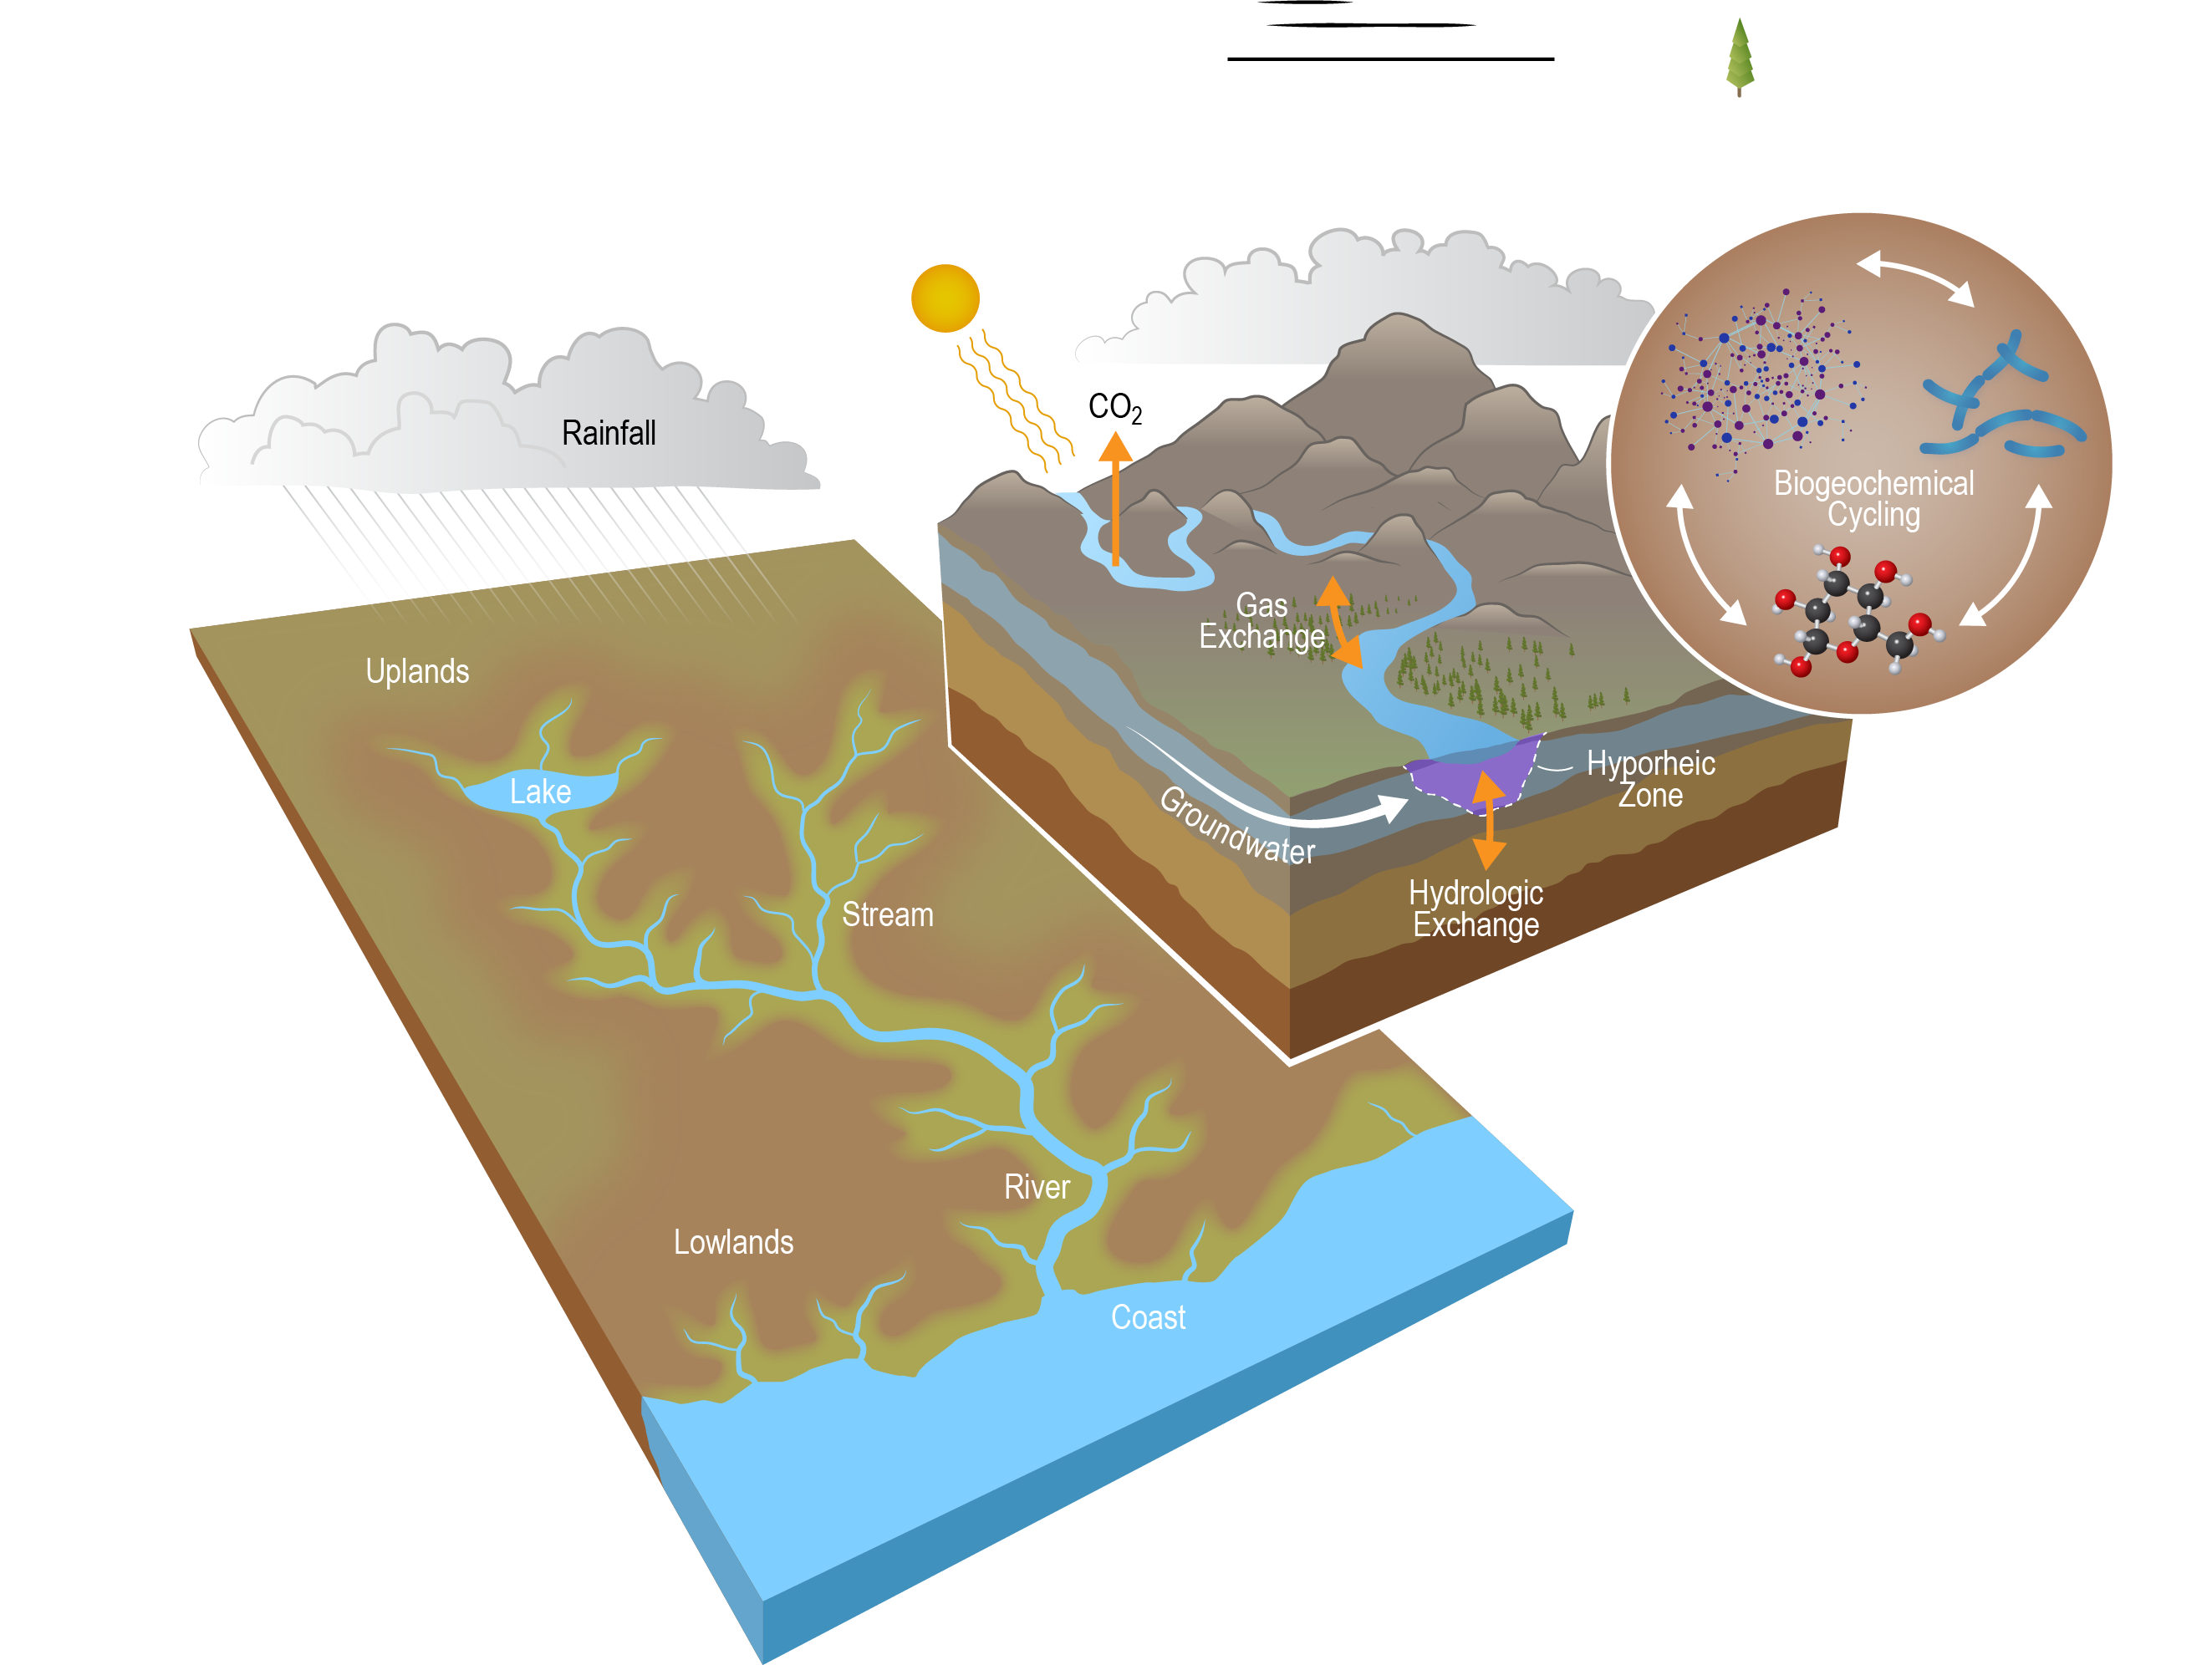
\includegraphics[width=1.0\linewidth]{EED0542_watershedModel.png}
\caption{Conceptual model of hydrologic and biogeochemical processes at the watershed scale.}
\end{figure}

Improving the understanding of how extreme events impact watersheds has become increasingly more critical as the occurrence of these extreme events are projected to be more frequent and more intense \citep{IPCC2012}. Watershed models are key tools for understanding watershed functions and their responses to perturbations, and thereby for managing water resources \citep{Weiler2004, Burt2005, Beven1997, Jones1993}. Mechanisms that well represent watershed hydro-biogeochemical responses to mild environmental stresses may not be extrapolated to represent responses to extreme events such as floods and droughts. Furthermore, the spectrum of environmental stresses that have been modeled is data sparse, especially with respect to extreme events. High variability in the relatively few end member observations, against which models are calibrated, results in high uncertainty in model conceptualization, which is ultimately translated into model structural error. Decreasing model structural uncertainty would better inform sustainable management of watershed systems under projected environmental stresses, which are critical for enhancing our economical and societal resilience \citep{Srinivasan2017, McDonnell2018b}.

%in silico representations of hydro-biogeochemical processes through additional input of data (i.e., data-driven approach) or by using a different modeling approach (i.e., deep learning-based approach), or a combination of the two. Additional field-based observations help resolve how water moves across landscapes, its residence time, and what the biogeochemical properties are along various flow paths during extreme events. 

The objectives of this review paper are to: (1) review the current status of watershed modeling and monitoring in understanding watershed hydro-biogeochemical processes and predicting water quantity and quality under perturbations; (2) identify the key knowledge and capability gaps; and (3) present a path forward to integrate modeling and observations to advance predictive understanding of watershed hydro-biogeochemical responses to perturbations.


\section{Current Knowledge and Gaps in Understanding Watershed Responses}

The response of water quality to extreme hydrologic events in a watershed is shaped by geology, topography, land use, and past environmental conditions \citep{Kaushal2018f,Kaushal2018g}. Interactions of hydrologic and biogeochemical processes in watersheds are inherently complex (Fig. 1). They are manifested over a variety of temporal scales and spatial scales from single microorganism to individual plants to landscape \citep{Wang2015}. Coupled hydrologic processes include precipitation, overland flow, evapotranspiration, variably saturated flow, and the movement and exchange of between the land surface, soil, and the underlying aquifers \citep{Yu2018}. Coupled biogeochemical processes include mineral weathering, cation exchange, photosynthesis, nutrient cycling within each hydrological compartments, sediment erosion, as well as transformation and exchange between those compartments. Understanding watershed biogeochemistry that controls key water quality signatures at broad spatial scales must account for not only how processes in different landscape patches (e.g., in upland, riparian zone, and wetlands) are regulated, but also how they interact as water travels across the watershed. Transport processes must be coupled with element-specific cycling across space and time to understand the contributions of landscape patchiness and hydrologic and biogeochemical connectivity (the connection and disconnection of disparate landscapes via surface and subsurface flows) in controlling stream and river water chemistry\citep{Harvey2015b}. Research has just begun to connect transport mechanisms with element-specific releases to surface water \citep{Bao2017b,Kaushal2018f}. 

\subsection{Watershed hydro-biogeochemical processes}

The depth and length of groundwater flow paths strongly control C and N cycling and the delivery of below-ground biogeochemical reaction products to surface water \citep{McDonnell2007}. High DOC exports have typically been associated with near‐surface hydrologic flow paths that intersect DOC rich forest floor and surficial soil layers in riparian or wetland locations \citep{Frank2000e,Inamdar2006}. Rising groundwater tables also contribute to increased DOC concentrations in surface waters, known as the “flushing” effect \citep{Creed2008}. Nitrate (NO3$^{-}$) exports from watersheds occur along both shallow and deep groundwater flow paths \citep{Laudon2018b,Inamdar2006,McGlynn2003}. Therefore, understanding the subsurface routing of water through a watershed is fundamental for explaining hydro-biogeochemical responses in surface water. However, the role of subsurface biogeochemistry in watershed responses to extreme events and chronic changes remains poorly understood.

Subsurface flow depends on precipitation thresholds. In one example \citep{Tromp-vanMeerveld2006}, it was shown that precipitation events exceeding the threshold of 55mm resulted in a hundred-fold increase in subsurface flow compared to subsurface flow changes that resulted from storms producing less than 55mm of precipitation. Storm flow can be partitioned as moving slower through capillaries in the soil matrix or (generally) faster through preferential pathways. Traditionally, such preferential pathways were conceptualized as conduit macropore networks in the soil matrix that re-route water to arrive at the stream at rapid speeds \citep{Beven1982}. Preferential flows also occur at the interface between shallow surface soil and an impervious layer (e.g., bedrock; \citealp{Freer2002, Graham2010, Hopp2009, Lehmann2007, McGlynn2003, Salve2012, Tani1997, Tromp-vanMeerveld2006a}). Soil pores and microtopography of the bottom impervious layer are hypothesized to fill, then water can spill over the bottom boundary layers and initiate preferential flow with a threshold response \citep{Tromp-vanMeerveld2006a}. More recent studies have also shown that preferential flow paths through weathered and fractured bedrock may contribute significantly to watershed water balance (e.g., accounting for more than 30\% of precipitation) \citep{Kosugi2006, Graham2010, Aishlin2011, Flinchum2018, Tromp-vanMeerveld2007}. Preferential subsurface flow influences the source, age, and timing of water, C, and N losses in many systems, with important implications to biogeochemical reactions, residence time, and routing to downstream ecosystems \citep{Lohse2009}. Changes in precipitation extremes will likely alter runoff pathways and groundwater recharge, which may in turn increase nitrate and DOC concentrations in both groundwater and other receiving waters. However, it is extremely challenging to mechanistically  capture such preferential flows across watersheds because there are few observations of such flow responses during extreme storm events, and subsurface domains, especially bedrock fractures, are not easily accessible. While isotopic signature and long-term mass balance experiments could provide valuable information for the mixture of flow paths, residence time, and contributions from various land use patterns, such measurements have not been acquired in many watersheds.
    
Plant canopy interception and root access to subsurface water for transpiration can also impact the water balance by altering the soil storage of water and material, consequently on water and solute availability including location and timing across the landscape \citep{Brauman2015}. Under drought or water-limited conditions, plants modulate the transpiration demands by controlling the opening of their stomata to avoid catastrophic failure. Empirically-derived wilting parameters are crucial in connecting soil water conditions to plant transpiration \citep{Fang2017b,Chen2008}. Eddy covariance flux tower measurements \citep{Baldocchi2001} provide valuable datasets to identify the connections between the ecohydrologic fluxes and their driving forces and understand the feedback mechanisms between processes. An information theory-based approach \citep{Goodwell2018a} has been recently applied to understand how forcing and feedback mechanisms are linked to ecosystem responses (water, carbon, and heat fluxes at the land surface) to different types of disturbances (e.g., rainfall pulses and drought) using process connectivity between environmental variables. Based on analyses performed on two transects of eddy covariance towers across elevation and climatic gradients at the Critical Zone Observatories (CZOs) in Idaho and California, \citet{Goodwell2018a} found that ecohydrologic fluxes along climate gradients respond differently to disturbances, with significant influence of heterogeneity in soil characteristics, topography, vegetation, and soil microbial activity. Accounting for deep groundwater dependence of ecosystems under water stress is especially important for managing dryland ecosystems to achieve water resources sustainability \citep{McDonnell2018b,Miller2010}.

Knowledge of unprocessed atmospheric nitrate in waters is important to assess forest health and water quality in watersheds. A recent synthesis \citep{Sebestyen2019} of nitrate isotope studies around the Northern Forest Region revealed that nitrate enters the forests from atmospheric deposition and sometimes rapidly moves to streams without being biologically processed. Especially during higher-flow events caused by either rainfall or snowmelt runoff, unexpectedly high levels of unprocessed nitrate flows to streams could occur over a brief time window. Too much nitrogen, termed “nitrogen saturation,” can change forest composition and mobilize calcium in soil, leading to declining forest health and water quality. The effect of nitrogen saturation could be amplified if extreme precipitation events continue to increase in frequency and magnitude. Understanding the fate of nitrogen produced in the air and transported to the land and river networks is currently lacking due to lack of long-term monitoring of nitrate isotopes \citep{Schlesinger2009}.

Hydrologic flow paths and runoff sources are critical for explaining the differences in dissolved organic matter (DOM). The concentration, composition, and sources of DOM were found to differ dramatically between base flow and storm event conditions during a three{-}year period (2008\textendash2010) in a forested headwater catchment in the mid{‐}Atlantic Piedmont region of the US \citep{Inamdar2011}. The aromatic and humic DOM constituents in river water increased significantly during storm events, attributed to the contributions from surficial sources such as throughfall, litter leachate, and soil water. Groundwater sources contributed a large fraction of the DOM constituents during base flow and were responsible for the high percentage of protein‐like fluorescence observed in base flow conditions. By studying multiple storm events, this same study \citep{Inamdar2011} also revealed that summer storm events produced the highest concentrations of humic and aromatic DOM, while such response was muted for winter storms. A large precipitation event following summer drought produced a complex DOM response; this was not observed for other similar storm events, confirming the dependence of response on past environmental conditions. 

The composition of DOM has a large impact on the watershed biogeochemical processes, as revealed in recent studies \citep{Stegen2018,Goldman2017a,Graham2017d}. Laboratory experiments and field observations have revealed that microbial activities and organic carbon (OC) characteristics regulate the underlying mechanisms of biogeochemical cycling in surface water and subsurface systems, such as aerobic respiration and denitrification \citep{Stegen2018,Goldman2017a,Graham2017d}. Understanding of the input and fate of DOM in river networks has undergone dramatic transformation over the past decade with the availability of new measurement technologies such as high-resolution mass spectrometry. Challenges exist in translating information about the relative composition of different DOM components to masses to enable a better understanding of (1) the coupling between DOM composition and microbial uptake and nutrient cycling, and (2) the role of DOM at the watershed level \citep{Inamdar2011}. These challenges result in conceptual uncertainty in translating the knowledge into model representations. Methods are lacking to propagate that conceptual uncertainty through an integrated hydro-biogeochemical model framework and evaluate its importance, thus failing to take full advantage of the information potential available through these transformative advances in characterization.
            
\subsection{River corridor hydrology and biogeochemistry}

Hydrologic exchanges between the surface water and groundwater creates hydrological, thermal, biological, and chemical gradients across the interface of these two water bodies, which have significant impact on human and environment health \citep{Bobba2012,Conant2019}. The interaction zone, broadly defined as the river corridor \citep{Harvey2015b}, experiences bidirectional exchange of water, energy and nutrient driven by static and dynamic pressure variations over the streambed \citep{Grant2018}. However, quantifying the exchange of water and chemicals of interest across this interface at watershed scale is hampered by limited data availability and integrated models have not been applied to a wide range of settings due to heterogeneities in the stream channels and aquifers \citep{Barthel2016}. As of today, the study of river corridor processes still faces the challenges identified in \cite{Harvey2015b} four years ago: 1) how to transfer small scale process knowledge to larger scale water quality and ecological response that are cumulatively affected by these small processes; 2) how to resolve the effect of heterogeneities of multiple origins on hydrologic exchange flows and fate of nutrients and contaminants in rivers; 3) how to understand river corridor functions by quantifying “hot spots and moments” and reactant delivery effectiveness by hydrologic exchange flows for biogeochemical processing of nutrients and organic matter; and 4) how to avoid potential measurement bias of hydrologic exchange fluxes.  These challenges have recently been reiterated in a review paper by \cite{ward2019}. For an improved understanding of biogeochemical transformation processes across this interface, high resolution monitoring is essential to determine the spatial and temporal variability of hydro-biogeochemical parameters \citep{Gassen2017}. On the other hand, hydrologic connectivity cannot be ignored when addressing watershed scale water quantity and quality \citep{Freeman2007,harvey2019connectivity}.  Low-frequency large precipitation and snow events with future climate change can contribute to a significant proportion of annual terrestrial dissolved organic matter input to drainage networks and to downstream, higher-order rivers, bypassing headwater streams due to higher stream velocities during these events \citep{Raymond2016}.


\subsection{Linking with microbial and biogeochemcial processes}
            
While it is often assumed that high resolution data generated by emerging molecular 
techniques can improve our understanding and predictions of biogeochemical cycling \citep{Rocca2015, Graham2016, Hall2018}, we have a poor understanding of the environmental contexts as well as the spatial and temporal scales at which these data types truly provide added value for predictive power of watershed function. Recent meta-analyses have demonstrated weak relationships between microbial genes and biogeochemical processes, highlighting a falsehood in the common assumption that molecular data is spatially and temporally representative of broader ecosystem function \citep{Rocca2015, Graham2016}. Molecular information is typically extracted from a gram or less of sediment at sparse (or a single) time points and detect both active and residual constituents. In contrast, watershed functions of interest are over much larger spatial domains at daily or even finer resolution when evaluating rapid responses to intensive hydrologic disturbances. Therefore, questions remain regarding the spatial scales and domains at which molecular information is valuable for informing reactive transport processes at the watershed scale, and how the importance of molecular data varies over time when the perturbation progresses. For instance, \citet{Graham2014} demonstrated seasonal disparities in the power of microbiome genes to explain N cycling rates, and \citet{Blinn1995} demonstrated that benthic organisms can require four months of recovery time following subsequent 12-hr disturbances. In such a situation, genetic information on microbial communities may provide significant insight into biogeochemical reaction rates. \citet{Good2018} have shown the utility of a genohydrology approach at monthly or longer timescales. 

High resolution molecular data may be most useful for improving predictive models in systems with high spatiotemporal variability, wherein microorganisms integrate over the short-term hydrologic history of the system (days to weeks) and metabolomic data reflect biogeochemical processing in real-time. Examples of such situations include hyporheic zones, perturbation responses, and high-frequency stage variability (e.g., hydropeaking, coastal, storm-driven). Hyporheic zones are a nexus of hydrologic mixing and biogeochemical hotspots, with spatiotemporal variability in chemical constituents \citep{Boulton1998, McClain2003, Harvey2015b}. Heightened heterogeneity in this zone can generate disconnects between microbial metabolism and ambient geochemistry, therefore deviating true biogeochemical rates from functional predictions based solely on hydrobiogeochemical data types. Perturbations may similarly decouple extant microbiomes from environmental conditions, therefore increasing the value of molecular insights on predictions of biogeochemical rates during perturbation. High-frequency stage variations can alter the spatial extent and mixing conditions of hyporheic zones as well as perturb multiple components of watersheds \citep{Song2018b,Shuai2019b}, creating an ideal system for maximal value in molecular data. 

\subsection{Watershed Functions under Mild and Extreme Perturbations }
        
Interpretations of watershed modeling studies under mild and extreme perturbation forcing remain uncertain for several reasons. First, water quality responses to observed perturbations vary depending on the intensity, duration, and magnitude of an event. Various numerical modeling approaches simulate well the hydro-biogeochemical responses to most events in the subsurface and surface water domains, though simulations of responses to extreme events continue to contain high uncertainty due to the chaotic nature of large-scale atmospheric circulation \citep{Shepherd2014}.A study of 35 tropical cyclones over the past 2 decades found that watershed stream export of nutrients and carbon after major storms can be storm-specific, depending on the mechanisms that mobilize the nutrients and carbon \citep{Paerl2018b}. For P, large storm flows may lead to its release from sediment in inundated wetlands that experience low-oxygen river water conditions that often occur after the passage of tropical cyclones.  P concentrations increased as flow increased, which magnified the total impact of the storm. However, N concentrations had a non-monotonic and generally negative relationship with flow, suggesting non-point sources from unique land use were dominant, while dissolved and particulate organic nitrogen did not correlate significantly with flow  \citep{Paerl2018b}. Second, there are difficulties in obtaining field observations and doing process-based studies. Currently, watershed models under extreme perturbation forcing have been data sparse due to the paucity of studies \citep{Kaushal2018g, Vidon2018}, and the high variability in the relatively few end member observations against which models are calibrated. Some particular extreme events have been well-documented, though not all systems (e.g., riparian zones) in the watershed are well-represented \citep{Vidon2018}. Third, there is uncertainty about future anthropogenic disturbance to the environment and how that impacts watershed hydro-biogeochemical processes. Nutrient and carbon flushing is largely dependent on previous accumulation, due in large part to changing land use \citep{Paerl2018b}. Models show that flood magnitudes can decrease significantly in large rivers downstream of dams \citep{Lu2017a}, impacting nutrient and carbon loads downstream.  The capacity for stream and river ecosystems to retain and transform nutrient pollution from landscapes can become "saturated" during floods unless nutrient pollution sources are reduced at the watershed scale \citep{Kaushal2018g}. Fourth, there is a lack of a consistent strategy in terms of monitoring methods to fully assess the large-scale impact of extreme events \citep{Vidon2018}. 

An ensemble of climate projections run for the conterminous US showed that a 1 degree $^\circ$C increase of global mean temperature can significantly increase 11\% and 17\% more land area experiencing changes in summer and winter runoff probability distribution functions, respectively, when estimated at the continental scale, though changes in sub-basin runoff suggests the emergence of new hydrology regimes dominated by changes in process variability, regardless of the emission scenarios \citep{Leng2016c}. The predicted change in runoff is larger than that in precipitation \citep{Leng2016c}. This underscores that understanding and predicting how, when, and where changes in the quantity and quality of water resources occur requires deep insight into the physical and biological mechanisms that govern the cycling and transport of water and elements across complex watersheds under a wide spectrum of environmental stresses.

\section{Watershed Monitoring}
  \begin{sloppypar}          
Hydrologic and biogeochemical monitoring of watersheds is broadly dispersed across agencies and individual research teams. While an exhaustive review of all efforts across the globe is beyond the scope of this paper, we provide a summary of major infrastructure within the US with the goal of emphasizing strengths and weaknesses of current efforts. For example, the U.S. Geological Services (USGS) has developed and maintains an expansive monitoring network (\url{https://waterdata.usgs.gov/nwis}) focused on surface water quantity and quality using in situ sensors (e.g., stream gauges, water quality sondes) and field-collected samples. A key attribute of the USGS network is that much of the data is freely available and is consistently structured and managed. This allows the USGS data to be used extensively for operational decision making, flood prediction/response, and basic research into watershed function. The USGS network is, however, biased towards larger rivers and the network is primarily above the head-of-tide. As such, there are gaps in the monitoring of low-order streams and tidal rivers. USGS has also established the National Ground-Water Monitoring Network (NGWMN) (\url{https://cida.usgs.gov/ngwmn/index.jsp}), which provides monitoring data from groundwater wells distributed across federal, state, and local agencies. 

Recognizing a need for consistent monitoring data across environmental contexts, the U.S. National Science Foundation (NSF) has established the National Ecological Observatory Network (NEON) (\url{https://www.neonscience.org/}) as an observational platform across all biomes of the US. Similar to USGS, NEON data are consistently generated and structured, and are freely available. NEON includes both terrestrial and aquatic components, and their data span everything from ecosystem fluxes to soil microbes to plant/animal communities to stream discharge. The use of consistent methods to generate and openly provide data are not unique to the USGS and NEON, but they are also not necessarily common across other monitoring efforts. It is important to recognize that NEON was not established to monitor watersheds per se, but rather to monitor terrestrial and aquatic environments in localized field sites distributed across biomes of the US. NSF funds other major field efforts as well, such as the long term ecological research (LTER) network, which includes elements of ecosystem monitoring and experimentation. Like NEON, the LTER network is not necessarily focused on watershed monitoring. Other efforts funded by the NSF are more watershed-oriented, in particular the CZO network (\url{http://criticalzone.org/national/}) that spans a number of watersheds across the US. Efforts within CZO sites span a broad range of watershed attributes, though they often emphasize the geology and geochemistry of the deep subsurface. The NSF-funded CUASHI effort (\url{https://www.cuahsi.org/}) is another critical capability within watershed science. CUASHI is a consortium of universities that serves integrated watershed data (e.g., water discharge and quality) and provides access to models (e.g., the national water model) and training in watershed science methods.

In addition to the USGS and NSF, The US Environmental Protection Agency (EPA) has significant monitoring efforts, such as their National Streams and River Assessment (\url{https://www.epa.gov/national-aquatic-resource-surveys/nrsa}) that focuses on the ecological state and water quality of streams and rivers within the US. The EPA efforts have less emphasis, however, on watershed hydro-biogeochemistry. The US Department of Energy (DOE) funds a network of 5 watershed test beds distributed across the contiguous US. They collectively span much of the watershed continuum from low-order headwater streams in Colorado, to mid-order streams Tennessee, Wyoming, and Georgia, to a high-order river in Washington State. Research within these test beds is highly integrative that includes both monitoring and experimentation associated with surface and subsurface hydrology, (bio)geochemistry, microbiology, plant physiology, and ecosystem processes. In addition, data-generating efforts in these test beds often focused on informing mechanistic hydrobiogeochemical numerical models, such as subsurface reactive transport codes. Among agency-funded efforts, the DOE test beds are relatively unique in their level of focus on informing predictive models, which contrasts with other efforts (e.g., NEON) designed primarily as observatories with less emphasis on informing models. 

Similar monitoring strategy and efforts exist across the globe to understand watershed functions. For example, Canada’s Water Office provides real-time, nation-wide stream gauge data (\url{https://wateroffice.ec.gc.ca/}). Canada has also formed a watershed research consortium (\url{http://cwn-rce.ca/project/canadian-watershed-research-consortium/}) that aimed to develop consistent monitoring programs across watersheds to enable improved understanding and decision making. Recently, more community-driven networks are emerging, such as StreamPulse (\url{http://pulseofstreams.weebly.com/}) that includes hundreds of datasets from across watersheds to evaluate stream metabolism.  The ‘internet of water’ (\url{https://internetofwater.org/}) that focuses on improving access to watershed data by linking data producers (e.g., USGS), data hubs (e.g., NGWMN), and data users (e.g., researchers and decision makers). Worldwide Hydrobiogeochemistry Observation Network for Dynamic River Systems (WHONDRS) (\url{https://whondrs.pnnl.gov/}) is another network initiated by the watershed science community to provide unique data resources with detailed molecular characterization, focusing in the river corridors impacted by dam operations.
\end{sloppypar}

Enhanced coordination and standardization in terms of data generating methods and data archive practices is a major need within watershed science. The USGS and similar efforts in Canada and other countries provide a model of coordination, consistency, and openness that all of watershed science should aspire to.
            
%Level of coordination and standardization varies among the networks.  For example, NEON is highly coordinated with standardized data and a single point of contact for all field sites. In contrast, the CZO and LTER networks (also funded by NSF) are not coordinated in terms of data generation, data archiving, or site management. The DOE-funded watershed test beds are somewhere in the middle in that they are linked conceptually with a focus on watershed hydro-biogeochemistry and often use the same or similar numerical models, but are not coordinated in terms of data generation. In collaboration with a DOE-funded data archive (https://ess-dive.lbl.gov/), the test beds are moving towards standardized data formats and archiving practices that ascribe to FAIR (Findable, Accessible, Interoperable, and Reusable) data principles.  

\section{Watershed Modeling Approaches}

%Here we briefly review some existing hydrologic and water-quality models and their underlying philosophy to identify needs and gaps for further model development to predict watershed functions under perturbations. 

Watershed models can be broadly thought of as being either empirical (data-driven) or  process-based (mechanistic), although in practice many models employ a combination of the two approaches. Empirical models link inputs (e.g., geomorphic properties, land use, precipitation) and outputs (response/state of a watershed) through observationally-derived relationships. Because such models do not attempt to explicitly quantify the underlying physical, chemical and biological processes that connect inputs with outputs, they usually require a small numbers of parameters and are computationally inexpensive to implement. Some examples of empirical models include the unit hydrograph and curve number method \citep{USDA1986} used to estimate runoff, and the Universal Soil Loss Equation \citep{Hudson1993} used to estimate soil erosion. Machine learning (ML)-based relationships are a form of empirical model, typically derived solely through analysis of large datasets without imposing physical constraints, and methods such as Artificial and Bayesian Neural Networks \citep{Committee2000, Dawson2001, Dawson1998, Dwivedi2013} are increasingly being used to simulate hydrologic processes. Empirical models can be useful in ungauged watersheds, but they are valid only under conditions (i.e., high-level watershed characteristics) similar to those under which they were derived. Thus care must be exercised to ensure empirical models are not used outside their range of applicability. This may strongly limit their suitability for predicting responses to extreme events, which by definition are outside the range of "normal" events on which empirical relationships are based on and may also lead to fundamental changes in hydrologic connectivity and other features that control watershed responses.

Process-based models attempt to impose physical, biological, and chemical principles (e.g, conservation laws or laws of mass action) on the mathematical formulae relating model outputs to inputs (often using ordinary or partial differential equations). In practice it is not possible to resolve processes based on first principles alone. Closure approximations must be introduced \citep{Wood2009}, usually resulting in effective parameters or constitutive relationships that must be inferred from observational data, thus blurring the line between process-based and empirical models. Ubiquitous spatial heterogeneity in watershed processes commonly renders such parameters spatially variable and scale-dependent. Among process-based models, so-called lumped models use simplified governing equations without explicitly accounting for spatial variability in inputs and parameters. Examples  include Stanford Watershed Model IV (SWM) \citep{Crawford1966}, TOPography based hydrological MODEL (TOPMODEL) \citep{Beven1997}, Hydrologiska at Vattenbalansavdelning model (HBV) \citep{Bergstrom1976}, Hydrological Simulation Program FORTRAN (HSPF) \citep{Development, Duda2012}. These models are easy to use and calibrate, computationally inexpensive, and most codes are open source. However, lumped watershed models can only simulate aggregated behaviors of a watershed system, for instance, the streamflow response at the watershed outlet. Lumped models require long-term monitoring data for calibration, and their heavy reliance on calibration limits their applicability to extreme events that fall outside the range of historical observations. 

Unlike the lumped models, process-based distributed models attempt to capture the spatial heterogeneity of system responses by using spatially-distributed parameters and inputs, while the set of governing laws/equations remain same for the entire domain, such as the shallow‐water equations \citep{Hirsch1988} and the Richards equation \citep{Richards1931} for surface and subsurface flows, respectively. FLUX-PHIM-BGC\citep{Shi2018} and RHESSys \citep{Tague2004d} models are good examples for distributed watershed simulators that couple hydrologic process, surface energy flux, vegetation and nutrient dynamics. FLUX-PHIM-BGC was extended from PHIM \citep{Qu2004}, a distributed hydrologic model that simulates the water flux from surface and groundwater and its interaction and stream routing. Later, FLUX-PHIM\citep{Shi2013} was developed to account for the spatial and temporal heterogeneity in surface energy balance. Finally, FLUX-PHIM-BGC was developed to account for vegetation dynamics and carbon/nitrogen cycling in soil and stream. In principle, a spatially discretized model of a system with spatially distributed parameters and inputs is expected to provide better predictions than its lumped counterpart. However, such distributed models also require significantly larger number of unknown model parameters to be specified or estimated. The parameter dimensionality could quickly become intractable when dealing with complex, coupled physical and biogeochemical processes over a large spatial domain. Consequently, the computational cost associated with parameter estimation for such high-dimensional, computationally expensive models has hampered the practical application of distributed watershed models \citep{Pokhrel2008}.

\subsection{Watershed simulators}\label{simulators}

A number of watershed simulators have been developed for water quantity and quality modeling at the watershed scale (e.g. \citealp{Daniel2011, Singh2005, Wellen2015, Migliaccio2007, Moriasi2012, Devia2015, Elliot2010, Gao2014}). While it is beyond the scope of this review to provide detailed characterization of all available watershed models, readers are referred to previous review papers for more information \citep{Wellen2015, Fatichi2016}. Given the focus of this review on ecohydrological and biogeochemical processes, here we focus on watershed simulators that represent coupled vegetation, hydrology, and biogeochemistry in both land and river systems within a watershed context. Thus, some popular models are not included in our discussion because they do not simulate biogeochemical processes pertinent to water quality predictions, despite their wide use in watershed hydrologic modeling. Such examples include the Hydrologic Engineer Center’s Hydrologic Modelling System (HEC-HMS), Topography Based Hydrological Model (TOPMODEL) \citep{Beven1997}, Variable Infiltration Capacity (VIC) model \citep{Liang1994,Hamman2018}, and the Distributed Hydrology Soil Vegetation Model (DHSVM) \citep{Wigmosta1994} are not discussed.  

                
 Specifically, the watershed water quality models that are reviewed here include: the MIKE SHE (Système Hydrologique Européen) model\citep{Ma2016, Jaber2012}, Hydrologic Modeling Fortran (HSPF)\citep{Duda2012}, Soil and Water Assessment Tool (SWAT) \citep{Neitsch2011, Arnold1998, Gassman2007}, Storm Water Management Model (SWMM)\citep{Huber2003, Cambez2008, Rossman2010}, Annualized AGricultural NonPoint Source model (AnnAGNPS)\citep{Bingner2018, Yuan2001}, Areal Non point Source Watershed Environment Response Simulation (ANSWERS) ANSWERS-2000\citep{Bouraoui1996}, Watershed analysis risk management framework (WARMF)\citep{Goldstein2001, Herr2012}, Regional Hydro-Ecologic Simulation System(RHESSys) \citep{Tague2004d}, The Penn State Integrated Hydrologic model (PIHM) coupled with biogeochemcial processes (Flux-PIHM-BGC) \citep{Shi2018}. Based on the models reviewed in previous studies, as well as the models that have been identified as useful tools to support Total Maximum Daily Load (TMDL) analysis \citep{Shoemaker2005, US-EPA2019}, we summarize and compare key hydrological and biogeochemical processes represented by those simulators in Table 1. 

                \begin{landscape}
                %\begin{center}
                 \begin{spacing}{0.5}\centering % line spacing
                \begin{table}
                \scriptsize

                %\resizebox{1.4\textwidth}{!}{
                %\begin{tabular}{m{10em} | m{10em} | m{10em} | m{10em} | %m{10em} | m{10em} | m{10em} | m{10em} | m{10em} }
                %\begin{tabular}{p{6cm} | p{5cm} | p{5cm} | p{5cm} | p{5cm} %| p{5cm} | p{5cm} | p{5cm} | p{5cm} }
                %\begin{tabular}{ l | l | l | l | l | l | l | l | l | l}
                %\begin{tabular}{ c | c | c | c | c | c | c | c | c | c}
                \begin{tabu} to 1.65\textwidth {  X[l] | X[l] | X[l] | X[l] | X[l] | X[l] | X[l] | X[l] | X[l] | X[l] }
                %\begin{tabularx}{\textwidth}{c|c|c|c|c|c|c|c|c|c}
                
                 \multicolumn{10}{l}{\textbf{Table 1} } \\
                  \multicolumn{10}{l}{Key  hydro-biogeochemical processes simulated in watershed water quality models.} \\
                  \toprule[0.4ex]
                 %\hline % use this instead of \toprule to remove thick line; Journal of Hydrology doesn't have thick lines in their tables
                 
                    \textbf{Model} & \textbf{AnnAGNPS} & \textbf{ANSWERS-2000} & \textbf{HSPF} & \textbf{MIKE-SHE} & \textbf{SWAT} & \textbf{WARMF} & \textbf{SWMM} & \textbf{RHESS\textsubscript{ys}} & \textbf{Flux-PIHM-BGC}  \\
                     \hline
                     \textbf{Landuse (primary)} & Agriculture & Agriculture & Multiple & Multiple & Multiple & Multiple & Urban & Multiple & Multiple \\
                     \hline
                     \textbf{Vegetation} & Crop growth & Crop growth & LAI & LAI and root depth & Biomass accumulation & Vegetation cover & Vegetation cover & Vegetation growth & Vegetation growth \\
                     \hline
                     \textbf{Surface infiltration} & SCS curve number & Green-Ampt equation & Philip equation &  Richards equation & SCS curve number or Green-Ampt equation & SCS curve number & SCS curve number or Green-Ampt equation & Philip and Green-Ampt equations & Richards equation \\
                     \hline
                     \textbf{Surface overland flow} & SCS curve number & Manning and continuity equations & Chezy-Manning equation & Saint Venant equations & SCS curve number & SCS curve number & SCS curve number or Green-Ampt equation & Net detention storage & Saint Venant equations \\
                     \hline
                     \textbf{Soil water infiltration/drainage} & Storage approach & Storage approach & Storage approach & Richards equation & Storage approach & Storage approach & Storage approach & Darcy equation & Richards equation \\
                     \hline
                     \textbf{Subsurface flow} & Darcy equation & Darcy equation & Empirical storage approach (lateral interflow and groundwater outflow) & Richards equation or linear storage approach & Kinematic wave storage model (lateral interflow) and linear storage approach (shallow groundwater) & Darcy equation & Darcy equation & Darcy equation (shallow groundwater) and linear storage approach (deep groundwater) & 2D Dupuit approximation \\
                     \hline
                     \textbf{Soil biogeochemistry} & N, P, and C & N and P & N and P & User-defined pollutants & N, P, and C & N, P, and C & User-defined pollutants & N and C & N and C \\
                     \hline
                     \textbf{Instream flow} & Manning equation & Manning and continuity equations & Continuity equation and  kinematic wave model & Saint Venant equations & Variable storage or Muskingum method & Manning and continuity equations & Saint Venant equations & Kinematic wave model & Saint Venant equations \\
                     \hline
                     \textbf{Instream biochemical constituents} & N, P, and pesticides & N and P & N, P, BOD, algae, and O\textsubscript{2} & User-defined pollutants & N, P, BOD, algae, O\textsubscript{2}, and pesticides & N, P, BOD, algae, and O\textsubscript{2} & User-defined pollutants & N/A & N/A \\
                     \hline
                     \textbf{Computing platforms} & Windows & Windows & Linux\textsuperscript{a, b} and Windows & Linux\textsuperscript{a} and Windows\textsuperscript{a, c} & Linux\textsuperscript{a} and Windows\textsuperscript{a, d, e} & Windows & Linux\textsuperscript{a, f} and Windows & Linux\textsuperscript{a} and Mac OS\textsuperscript{a} & Linux\textsuperscript{a}, Windows\textsuperscript{a}, and Mac OS\textsuperscript{a} \\
                     %\hline % use this instead of \bottomrule to remove thick line
                     \bottomrule[0.4ex]
                
                % footnotes listed on individual lines:
                %\multicolumn{10}{l}{\textsuperscript{a}Capable of High-Power Computing (HPC) on multiple cores} \\   
                %\multicolumn{10}{l}{\textsuperscript{b}\citealp{Kim2019}} \\
                %\multicolumn{10}{l}{\textsuperscript{c}\citealp{DanishHydrologicInstitute2019}} \\
                %\multicolumn{10}{l}{\textsuperscript{d}\citealp{Zhang2013}} \\
                %\multicolumn{10}{l}{\textsuperscript{e}\citealp{Rouholahnejad2012}} \\
                %\multicolumn{10}{l}{\textsuperscript{f}\citealp{Burger2014}}
                
                % footnotes listed altogether:
                \multicolumn{10}{1}{\textsuperscript{a}Capable of high performance and parallel computing; \textsuperscript{b}\citealp{Kim2019}; \textsuperscript{c}\citealp{DanishHydrologicInstitute2019}; \textsuperscript{d}\citealp{Zhang2013}; \textsuperscript{e}\citealp{Rouholahnejad2012};} \\ \multicolumn{10}{l}{\textsuperscript{f}\citealp{Burger2014}} \\
                

                %\end{tabular}
                \end{tabu}
                %\end{tabularx}
                \end{table}
                %\end{center}
                \end{spacing}
                \end{landscape}
                
As shown in Table 1, those popular watershed models vary widely in terms of process complexity and algorithms used to solve different processes. In general, all watershed models linked plant growth with hydrologic and water quality processes. Most of them used prescribed crop characters (e.g. Leaf Area Index -- LAI), instead of explicitly simulating the dynamic plant growth processes. Simulators also have their unique development histories. Each simulator has distinct strengths in solving different problems owing to different assumptions that were made during the construction of various model architectures. Although SWAT dynamically simulates plant growth and development as regulated by climatic (e.g. temperature) and environmental (e.g. nutrients availability), its representation of forest growth processes are oversimplified \citep{Yang2016}, making it unsuitable for simulating forest management. However, RHESSys \citep{Tague2004d} included a carbon cycling model adapted from BioME-BGC \citep{thornton1998regional} with litter and soil organic matter decomposition and nitrogen cycling model \citep{parton1996generalized} to simulate dynamic vegetation responses to climate, soil moisture and nitrogen conditions. Similarly, FLUX-PHIM-BGC \citep{Shi2018} also can simulate the spatial and temporal variation of LAI across landscape by adapting carbon cycling module from BioME-BGC.

As to surface runoff, soil water, and ground water simulation, the existing models use very different approaches, ranging from empirical methods to physically based equations. Most models (except SWMM and MIKE-SHE and FLUX-PHIM-BGC) use Manning’s equation or other simplified forms of the St. Venant equation rather than its dynamic wave version to improve computing efficiency. Among the 9 models, HSPF, SWAT, and WARMF explicitly represent soil N and P cycles and simulate reactive transport of N and P through channels, while other models use simplified approaches to simulate coupled land and channel cycling of water quality constituents. 

We also review whether those simulators have been adapted to High Performance Computing (HPC) given the increasing complexity and computational demand of watershed models. Most of the simulators have not been adapted to HPC except for RHESSys, FLUX-PHIM-BGC, and MIKE-SHE. RHESSys and FLUX-PHIM-BGC adopted the openMP library for paralell computing. MIKE-SHE, the only non-public domain simulator reviewed here, has implemented algorithms to leverage Graphical Processing Units (GPUs) in addition to central processing unit (CPU)-based parallelization. The channel routing component of SWMM has been parallelized to solve the Saint Venant equations. Although HSPF and SWAT have not been parallelized yet, they can be run on linux clusters to facilitate parameter estimation in parallel mode. Generally, models that offer a graphical user interface are not capable of code parallelization for shared and distributed memory platforms. 

\subsection{Emerging modeling trends, gaps, and challenges}

 Recently there has been growing emphasis on including integrated surface-subsurface flow, biogeochemistry, and land surface (including plants) processes to simulate watershed functions. To properly simulate the biogeochemical cycling of carbon, nutrients, and metals within the watershed systems, it is essential to couple integrated hydrological processes across the atmospheric upper boundaries to the bottom of bedrock with vegetation dynamics and mechanistic carbon/nitrogen cycling. Representing the increasing complexity of coupled processes using physics-based approaches are becoming more and more practical with dramatic advances in computing powers nowadays.  
 
 The response of water quality in receiving streams to any perturbations including extreme hydrologic events (perhaps occurring elsewhere in the watershed) is shaped by many factors, including geology, topography, land use, and historic regimes of environmental conditions (e.g., climate and nutrient loading) in the watershed. These factors vary widely and nonlinearly across spatial and temporal scales, which make it difficult to model numerically. Hydrological events \citep{Lu2017a} and therefore reaction zones \citep{McClain2003} can be highly localized in the watershed. An accurate characterization of watershed biogeochemistry must account for not only how hydro-biogeochemical processes are regulated within different localized landscape patches (e.g., in upland, riparian zone, and wetlands), but also how they interact as water travels through these often heterogenous patches \citep{Laudon2018b}. Most existing watershed models do not dynamically link groundwater and surface water or consider the transition zones between these two water bodies. Moreover, the limited models to study hyporheic exchange and nutrient cycling often assume steady state and static pressure variations. However, anthropogenic activities are known to induce high-frequency variations that enhance the hydrologic exchange flows and the associated heat exchange and biogeochemical reactions \citep{Shuai2019b,Song2018b}, which have not been accounted for in existing watershed models.
    %Accurate simulation of hydro-biogeochemical processes in numerical models is challenging due to the highly non-linear flow response during and immediately after a storm event, as well as how to represent the scale dependent processes.
    
Current-generation watershed water quality models do not fully incorporate emerging hydro-biogeochemical process understanding because of challenges associated with multi-scale heterogeneity, large spatial scale, and computational and characterization burdens. As a result, those models are of limited use for extrapolating from current environmental conditions to understand how watersheds will respond to land-use change and atmospheric perturbations. At the same time, there is still ongoing debate on how much complexity can be supported by data \citep{Jackson-Blakea}. Most watershed water quality models \citep{Kaushal2018f, Vidon2018} do not incorporate multicomponent reactive transport, which limits their ability to accurately predict distinct mixtures of water quality constituents \citep{Kaushal2018f} as a result of complex interactions between climate variability and human-dominated land use. The lack of biological and reactive transport processes in watershed models will likely lead to uncertainty and bias in predicting watershed C and N responses. The incorporation of fine-scale mechanistic understanding into a watershed biogeochemical model remains untested, but it has great potential predictive power to capture distinct water quality signatures and sources for multiple elements and chemical species across variations in land use, underlying geology, atmospheric deposition, and climate. 
    
While hydrologic connectivity, flow path characteristics and distribution, and watershed transit times are key controls on watershed biogeochemical processes, suitable measures and model estimation procedures for these key variables, including the diagnosis of source area contributions \citep{Hewlett1967}, have not yet been devised and are lacking, especially regarding responses under extreme climate events. Subsurface flow and transport, a primary vector for water flow and material transformations in watersheds with long residence times, is often oversimplified in watershed models. It has been documented that no explicit representation of lateral flow, common in land-surface models, led to overly spiky behavior in watershed hydrographs \citep{Clark2015d}. Explicit representation of topology and subsurface transport pathways within models will lead to dramatic improvements in watershed-scale biogeochemical understanding and prediction.
    


%Watershed studies incorporate theory that characterizes fate and transport mechanisms at smaller scales (e.g., pore, hillslope, and stream reach scales), which are then upscaled to the larger watershed scale \citep{Boano2014, Sivapalan2003}.

%Several formidable challenges inhibit the predictive understanding of watershed hydro-biogeochemical functions across spatial and temporal scales. First, transferring information from one scale to another is a problem because of the scale discrepancies between observations and models. For example, watershed models require high temporal resolutions of precipitation data for accurate partitioning between runoff and infiltration \citep{Guo2018}, but the temporal resolutions data are typically not available at sub-hourly temporal scales. Second, ground-based monitoring (e.g., permeability, and discharge) can be expensive and, hence, is limited to a few locations in a watershed. Nevertheless, predictive models require well-sampled data across the modeling domain; filling gaps in the sparse data is essential and exceptionally challenging. However, novel measurement techniques (e.g., high-resolution remote-sensing products) may be able to address scale discrepancies between models and measurements in the future (e.g., see some examples of new data in \citep{Hubbard2018}). \\
                 
Scaling remains as a persistent challenge in watershed hydrology and biogeochemistry \citep{Bloschl1995, Scheibe1998, Bras1999, Das2008, Li2008, Crow2012, Gentine2012, Arora2015, Dwivedi2016, Dwivedi2016a, Dwivedi2017,McDonnell2007}, partially due to the intrinsic complex nature of the coupled processes and the  computational tractability to capture enough complexity in reality. High-resolution watershed models are computationally expensive and require boundary conditions and forcings defined at the corresponding resolution to capture the nonlinear behavior. In contrast, coarse-resolution watershed models are computationally more affordable but do not adequately resolve finer-scale heterogeneity; thus, they are likely to misrepresent critical processes. Ideally, multi-scale process representation can be a way to demonstrate the ability of watershed models to reproduce processes across scales. Integrating multi-scale information into models will reproduce processes at their native resolutions, which can be a viable strategy for circumventing downscaling/upscaling needs. It is important to note that the term “scaling” has several uses, such as the estimation of intervening values from sparse data, aggregation or disaggregation of information by taking areal averages, and information transfer from small to larger areas \citep{Western2002}. Upscaling permeability presents such an example, where point scale measurements are used to infer effective permeability values at different scales. To illustrate further, the Richards equation was derived to represent the column-scale water movement, and it is used in several watershed simulators, as described in Section \ref{simulators}. Although these simulators are still useful at the watershed scale, scale-dependent parameters are required for acceptable functional behavior \citep{Western2002}. 

The literature contains several different approaches to link parameters and state-variables across different scales \citep{Bloschl1995}. In this context, the Miller--Miller similar media theory has been widely used to scale soil hydraulic properties as well as flow and transport equations \citep{Miller1956, Sadeghi2016}. Other researchers subsequently developed techniques to derive effective hydraulic properties using stochastic, fractal, or scaling invariant approaches \citep{Russo1993, Mohanty2000, RodriguezIturbe1998}. These techniques have also been used to understand the scaling characteristics of other hydrologic aspects such as drainage patterns, stream networks, and topography \citep{Gupta1990, Sivapalan2011}. The extension of the Miller--Miller similar media theory is the representative elementary area/watershed and Reynolds’ averaging concepts, assuming that the physics are known at the smallest scale considered. These concepts have primarily been used to define the physically meaningful control volumes at which hydrologic processes operate and give insights into understanding large-scale processes \citep{Wood1988, Reggiani1998, Reggiani1999, Reggiani2001}. The representative hillslope is an example of one such meaningful control volume in watershed science, which has been widely used to understand precipitation runoff, infiltration, and other key hydrologic processes \citep{Troch2003, Troch2015, Hazenberg2015, Hazenberg2016a}. Biogeochemical scaling is still in its infancy. There are a few examples that have used dimensionless numbers (e.g., Damk\"ohler numbers), Bayesian methods, and scale-dependent rates to upscale geochemical concentrations and fluxes \citep{Gu2007, Li2008, Arora2015, Dwivedi2016a}. However, we will conclude here by mentioning that hydrologic processes mediate biogeochemical processes; therefore, resolving hydrologic scaling should be key in efforts to address biogeochemical scaling issues.

Despite of insights offered in the literature, the fundamental problem remains the limited predictive understanding of hydrobiogeochemical systems at the watershed scale due to the lack of a unifying theory of hydrologic scaling. In fact, there may not exist any single universal relationship of hydrologic processes, given the inexact nature of hydrologic science \citep{Bloschl1995, Beven2006a}. Notwithstanding these issues, it is possible to develop scaling laws or strategies to enhance predictive capabilities using watershed models. Here we want to identify key issues related to distributed parameter models and give directions for future research.


\section{Watershed Model and Data Integration}

Extensive efforts have enhanced the mechanistic foundation of process-based watershed models in capturing interacting physical and biogeochemical processes while also making them spatially distributed to represent the spatial heterogeneity in parameters and inputs \citep{Wellen2015}. The development of increasingly mechanistic models is accompanied by concerns of overparameterization, equifinality \citep{Jackson-Blakea, Beven1992b, Beven2006}, and difficulties in estimating valid, spatially-distributed model parameters and driving forces \citep{Kollet2008b, Samaniego2010, Montanari2012, Raleigh2015, Raleigh2016a}. Some inputs (forcing and parameters) can be determined through direct observations in the field, whereas others are inversely estimated using the input-output records of the watershed. The best practices are recommended to include sensitivity analysis, optimization/calibration, validation, uncertainty analyses, and quantification of fit \citep{Chapra2008b}. However, the increasing computational cost of high-resolution mechanistic watershed models inhibits the broad community from following the best practice to improve process-based models. It is an even bigger challenge for models targeting the watershed responses under extreme events \citep{Wellen2015}. Most model calibration practices often rely on single-point, sparse time-series observations \citep{Wellen2015, Robson2014b}, which does not account for all the information that is contained in spatiotemporal observation data, and at the same time, it could lead to preference over simpler models. Considerable uncertainty exists in conceptualizing (i.e., selecting processes and their associated mechanisms for all the compartments and interfaces and parameterizing a process-based watershed model \citep{McDonnell2007, Duncan}. A multi-model approach called the Structure for Unifying Multiple Modeling Alternatives (SUMMA)\citep{Clark2015d, Clark2015a} framework has been explored for hydrologic models \citep{Clark2015d, Fenicia2011c, Clark2008b} to evaluate various conceptualization decisions in a systematic and controlled way. By doing so, modelers can select among multiple alternatives to improve model fidelity and pinpoint specific reasons for model weaknesses to prioritize research and development needs. 
    
It is recently argued that the success of data-driven machine learning methods relative to process-based modeling indicates that there is unused information in observation data \citep{Nearing2018c}. A more rigorous way of dealing with uncertainty is to pose it in terms of information, i.e., asking the questions of “how much information do we have and how well do we use it? \citep{Nearing2018c}” In this context, improving a model is about assimilating information (or learning) from both observations and models, thus establishing a theoretical linkage with the Bayesian learning based on the Bayes’ theorem. Using a Bayesian learning framework, classical questions in watershed modeling such as scaling, heterogeneity, and complexity can all be posed in terms of information and learning. 

Sensitivity analysis is a vital tool in numerical modeling for quantifying contribution of uncertainty from various sources to the overall uncertainty in model predictions \citep{Dai2017a, Dai2017, Razavi2015, Gupta2018}. Conventional global sensitivity analysis methods \citep{Saltelli2000, Chu-Agor2011, Song2015b} focus on the importance of model parameters. They are insufficient for identifying dominant model processes, each of which usually consists of multiple parameters \citep{Clark2015d, Clark2015a}. Process-oriented sensitivity analysis has gained increasing attention for improving hydrological models and beyond \citep{Dai2017, Sivakumar2004e, Sivakumar2008b}. A recent advancement in sensitivity analysis is to quantify uncertainty contribution from multiple, spatially-distributed model inputs using a simple, three-layer structure of uncertainty: model parameters, model structures, and forcing scenarios. Recognizing that a three-layer structure is too restrictive to describe the large number of uncertainty sources involved in multi-process environmental modeling and their complex relationships, a new sensitivity analysis method was developed based on the concepts of Bayesian networks (BNs) \citep{Heckerman1997c, Velikova2014, Pearl1988} to account for the complex hierarchical uncertainty structure of a model system \citep{Dai2019}. This BN-based sensitivity analysis method uses a graphical representation to propagate uncertainty with Bayesian inference, i.e., deriving joint probabilities. It affords substantial flexibility to quantify uncertainty contribution from a group of inputs, which is not possible without BN. 

Transformational advances in watershed modeling capabilities are facilitated in part by dramatic increases in the amounts, quality, and coverage of relevant observational data, but new challenges exist in harnessing big data \citep{Uddameri2018,Rosenberg2014}. Importantly, coordinated efforts by many governmental agencies over the past few decades have resulted in widely available datasets with extensive or even seamless spatial coverage. In the United States, data availability and interoperability have been advanced through a number of initiatives.  The U.S. Office of Management and Budget published Circular A-16 in 2002, which ``provides direction for federal agencies that produce, maintain, or use spatial data either directly or indirectly in the fulfillment of their mission and provides for improvements in the coordination and use of spatial data.'' Further coordination was spurred by the U.S. Office of Science and Technology Policy (Subcommittee on Water Availability and Quality) through the Open Water Data Initiative started in 2014 \citep{Bales2016, Maidment2016}. These coordinated efforts over the past two decades have led to critical data products such as the National Hydrography Dataset (NHD), the Watershed Boundary Dataset (WBD), and NHDPlus (an enhanced version of NDH). \cite{Fatichi2016} describe several other sources of freely-available internet-accessible spatial datasets including soil survey, precipitation, meterological forcing, river morphology and hydrogeologic property data. Remotely-sensed data such as those provided by NASA's Earth Observing System (https://eospso.nasa.gov/content/nasas-earth-observing-system-project-science-office) further expand data types to include vegetation and land use/land cover, soil moisture, changes in groundwater levels, and many others.
            
Work is ongoing not only to increase data availability, but also to break down barriers to effective use of these data in model development. A key challenge is posed by the diversity of data formats, locations, and modes of access, which often requires a large time investment in data compilation and formatting during model construction. Efforts to address this challenge include development of standardized data models \citep{Hu2015, Abdallah2019}, open source tools for data retrieval and preprocessing such as HydroDesktop \citep{Ames2012}, HydroShare \citep{Horsburgh2016} and the Observatory for Gridded Hydrometeorology \citep{Phuong2019}, and methods for linking Geographical Information Systems (GIS) with process-based models in loosely-coupled \citep{Alcaraz2017}, tightly-coupled \citep{Bhatt2014}, and seamlessly-coupled \citep{Wang2016} approaches. 
            
These advances not only enable better and more efficient development of process-based distributed hydrologic models, but also can lead to enhanced collaboration \citep{Bandaragoda2019}, improved reproducibility of published results \citep{Stagge2019}, and broader adoption of open science in practice \citep{Yu2016}. Automated model setup and execution based on open data, while necessarily subject to careful evaluation, could dramatically increase model accessibility and is moving from vision to reality (e.g., \cite{Starn2018, Lewis2018}).


\section{Going Forward: Systematic extraction of information from both observations and modeling for learning watershed systems to reduce uncertainty}
    
Bayesian Networks possess great potential to unite data-driven and process-based modeling approaches to identify and extract the most useful information out of observational data and predictive models. Th new BN development, combined with the wide adoption of Bayesian-based inverse modeling, parameter estimation, data assimilation, and model diagnosis \citep{Rubin2010b, Chen2013a, Chen2012a, Nearing2018c, Liu2007b, Gupta2008, Over, Simmons2016, Ye2004, Joseph2013, Gelman2014c, Nearing2016}, suggests a new and potentially powerful Bayesian framework can be built to unite sensitivity analyses, data assimilation, inverse modeling, and model intercomparison/diagnosis under the Bayesian theory for systematic data-model fusion under both data and model uncertainty. BN will allow the integration of deep learning methods \citep{Sun2019, Sun2018, Shenc, Gentine2018, Reichstein2019} to discover unknown physics where process understanding is lacking. Such a framework, as in the proposed research, would transform our learning process for watershed modeling by enabling us to answer questions like “What do we know about the system, how well are we translating that knowledge into predictive power, and how can we be more predictive?” Hence, to continuously improve predictive understanding. The data-model fusion will advance the fundamental understanding of hydro-biogeochemistry in watershed systems by iteratively asking questions like “What do we know about the system; How well are we translating that knowledge into predictive power; and How can we be more predictive?” and answering them with integrated sensitivity analyses, data assimilation, and mutual information analyses. Such systematic learning from data and models will not only lead to a new modeling capability for forecasting water quality and quantity in watersheds of various scales and land use patterns; it can also guide design of monitoring networks and experiments to collect the most valuable information to reduce uncertainty in predictive models. Ultimately, the data-model integration will link best-in-class modeling capabilities with the multi-agency long-term monitoring efforts to meet society’s needs under a changing environment, thus providing transferable scientific tools to help manage vital watershed systems for sustained water security and human and ecosystem health.

\subsection{Enhancing model-guided multi-scale observations}
    There are many paths forward for future integration of more and better data into process-based numerical models. One is the collection and analysis of isotope data. Historically, isotope hydrologists utilized environmental and artificially labeled radioactive isotopes (e.g., Ra, \textsuperscript{3}H, \textsuperscript{14}C, \textsuperscript{24}Na, \textsuperscript{82}Br, and \textsuperscript{32}P) to measure physical processes, such as stream discharge, groundwater direction, velocity, and age, and sediment loading at the reach or regional/aquifer scale \citep{Joly1922, Agency1963, Agency1967} before broadly switching to utilizing conservative transport of stable isotopes (e.g., \textsuperscript{2}H, \textsuperscript{18}O, and \textsuperscript{13}C) to infer other things, such as flow path characteristics \citep{Klaus2013}, water transit times \citep{McGuire2006}, weathering \citep{Schulte2011}, and water \citep{Agency} and carbon \citep{Dawson2011} balances at the watershed scale. More recently, reactive transport of stable isotopes of nitrogen (\textsuperscript{15}N) and phosphorus (\textsuperscript{18}O in PO\textsubscript{4}) have been utilized to identify non-point sources of anthropogenic N \citep{Fry1999, Lake2001, Spoelstra2001, Robinson2001, Mayer2002, M.JakeVanderZanden2005, Kendall2008, Savard2010, Nestler2011, Kaushal2011} and P loading \citep{McLaughlin2006, Elsbury2009, Paytan2012, Granger2017, Tonderski2017, Ishida2019}, and, later, elucidate specific biogeochemical processes, such as dilution \citep{Archana2018}, nitrogen assimilation \citep{Deutsch2009, Nikolenko2018}, denitrification \citep{Wexler2014}, phosphorous release from anoxic sediments \citep{Elsbury2009}, and cellular metabolism in aquatic food webs \citep{Davies2014} at various spatiotemporal scales.
            
    Now, isotope data are increasingly coupled with or incorporated into numerical models, which further augment the ability of these models to simulate complex physical processes with high precision. Such processes include groundwater flow dispersion \citep{Cornaton2011, Jiang2019}, preferential flow partitioning \citep{VanderHoven2002, Dusek2018}, surface/subsurface water mixing \citep{Turner2006}, nitrification and denitrification \citep{Choi2003, Chen2004, Rutting2007}, and anammox \citep{Granger2016}. The use of chemical and isotopic tracers has moved out of the field of chemi-hydrometry \citep{Groat1915} to isotope hydrology \citep{Agency} to hydrogeology and geochemistry \citep{Agency1974}, and now, to hydro-biogeochemistry and process-based numerical modeling.  Watershed modelers will continue to require more isotope data to feed into their models and many current monitoring networks serve as suitable infrastructure for collecting such data. 

    %More recently, Berkeley Lab's Scientific Focus Area (SFA) is studying how watershed function and respond to perturbations such as early snowmelt \citep{Hubbard2018}. The SFA has demonstrated the value of using multi-scale observations, from the canopy to bedrock, and high-resolution mechanistic models to explore watershed behavior and its response to disturbances \citep{Carroll2019, Dwivedi2017, Dwivedi2018}.  Efforts are underway to develop the understanding and tools to predict watershed response at the large scale ($\sim$300 km$^2$) and downstream river water quality.
    %In fact, RS technologies have become invaluable tools for watershed-scale modeling and analyses, particularly in conjunction with the advancement of spatially distributed hydrological models \cite{Dwivedi2016}. Yet these physics-based distributed models require extensive amounts of data to both parameterize and provide boundary conditions to simulate watershed processes \cite{Asger2001}. In fact, RS technologies have become invaluable tools for watershed-scale modeling and analyses, particularly in conjunction with the advancement of spatially distributed hydrological models \cite{Dwivedi2016}. Yet these physics-based distributed models require extensive amounts of data to both parameterize and provide boundary conditions to simulate watershed processes \cite{Asger2001}. 

On the other hand, remote sensing (RS)—in the context of watershed science—is the science and art of acquiring information about the land surface and subsurface or physical processes using remotely located sensors \cite{ritchie1996remote}. A diverse set of RS techniques exist to collect above- and below-ground data. RS relies on active and passive sensing technologies. Active sensors emit energy to examine part of the watershed (i.e., target), while passive sensors detect the radiation emitted from the target. After acquiring signals, various algorithms have been developed to translate them into surface and subsurface properties as well as hydrological and biogeochemical variables. The quality of RS data depends on its spatial, temporal, and spectral resolutions. More information about RS can be found in the literature \cite{Arora2019,  entekhabi2010soil, fonstad2013topographic, li2008effect, turner2004scaling,  zhang2003progressive}. RS provides a means to acquire spatial data and characterize their heterogeneity at the watershed scale. On the contrary, conventional methods are primarily limited to point measurements and incapable of providing adequate data to represent the heterogeneity of the land surface and subsurface properties reasonably. Therefore, the use of RS data has the potential to transition data-poor to data-rich environments needed for advancing watershed science. The use of RS in hydrology is not new, and its potential was revealed very early. In 1965, Walter Langbein, a pioneer of watershed science, advocated for the use of satellite platforms for acquiring hydrologic data, while RS techniques could measure soil temperatures, water vapor, and radiation using aircraft platforms \citep{Langbein1965}. \citet{ragan1980runoff} subsequently used curve numbers and land use mapping (Landsat product) to quantify runoff \citep{ragan1980runoff}. More notably, \citet{beven1979physically} demonstrated the importance of topography in predicting runoff using digital elevation maps. Since then, numerous articles published in the literature have used RS products to describe and characterize different aspects of watershed science, such as soil moisture, surface temperature, landcover/vegetation, precipitation, snow depths and cover, and groundwater \citep{fonstad2013topographic, hutengs2016downscaling, li2008effect}. 

We can now see every component of the water cycle remotely: precipitation, snow, evapotranspiration, surface soil moisture, deep groundwater, and river discharge (e.g., \citealp{Andreadis2017}). For rainfall, the Tropical Rainfall Measuring Mission (TRMM) at the turn of the millennium \citep{Kummerow1998} eventually evolved into the Global Precipitation Measurement (GPM) constellation \citep{Smith2007}; CloudSat has also provided complementary measurements of precipitation \citep{Stephens2002}. We have been able to see snow cover from the MODerate resolution Imaging Spectroradiometer (MODIS), with approaches to derive snow water equivalent (SWE; \citealp{Hall2002}); airborne capabilities such as the Airborne Snow Observatory (ASO) can assess SWE with high fidelity using LiDAR and can complement the snow depth measurement with albedo used for melt rates \citep{Painter2016}. Evapotranspiration has been derived from Landsat, the Advanced Very High Resolution Radiometer (AVHRR), and MODIS for decades \citep{Fisher2017}, and the ECOsystem Spaceborne Thermal Radiometer on Space Station (ECOSTRESS) on the International Space Station was designed specifically to focus on evapotranspiration at very high spatial and temporal resolutions \citep{Fisher2019}. A snapshot example of evapotranspiration over the Columbia River Basin in the US is shown in Figure 2.

\begin{figure}[hp]
\centering\includegraphics[width=1.0\linewidth]{ECOSTRESS_Columbia_River_Basin.png}
\caption{Evapotranspiration over the Columbia River Basin in the US from ECOSTRESS. The data show variability across the basin as well as fine-scale heterogeneity (70 m resolution) associated with landscape fragmentation and agricultural water use. Blue colors indicate high evapotranspiration (W m\textsuperscript{-2}) at the time of overpass (12:08 PM local time on June 14, 2019), and beige colors indicate low evapotranspiration.}
\end{figure}

The Soil Moisture Observing System (SMOS) and Soil Moisture Active Passive (SMAP) missions have provided global coverage of surface soil moisture \citep{Kerr2001, entekhabi2010soil}; airborne measurements provide increased depth and canopy penetration \citep{Colliander2017}. The change in deep groundwater storage can be derived through gravity-based measurements of total water storage from the Gravity Recovery and Climate Experiment (GRACE) and GRACE Follow-On (GRACE-FO) missions \citep{Rodell2002, Sheard2012}; global positioning systems \citep{Argus2014} and measurements of surface deformation \citep{Farr2014} can also be used to derive changes in groundwater. Finally, LiDAR can be used to measure river (and lake, reservoir, and ocean) heights, which can be used to infer river discharge; the airborne Surface Water and Ocean Topography (AirSWOT) has established the foundation for the upcoming satellite SWOT mission \citep{Durand2010}. Space agencies throughout the world continue to develop new missions to advance remotely sensed hydrological measurements, and the future will contain an even richer assessment of the hydrological cycle from space \citep{NationalAcademiesofSciences2018}. 

Although RS products are currently primarily used to characterize watershed properties for hydrologic processes, efforts are underway to derive biogeochemical properties (e.g.leaf chemistry) based on geomorphology and vegetation characteristics using hyperspectral data \cite{falco2019investigating} as well as to understand the subsurface physical properties of the watershed using  airborne electromagnetic (AEM) survey \cite{Hubbard2018}. Overall, RS promises massive data on every aspect of watershed science. A fusion of distributed hydrologic models and RS will take watershed science to the next level in the future.
            
Additionally, US DOE's Biological and Environmental Research (BER) office manages unique user facilities that can generate genomics and molecular-level data that are highly relevant to understand watershed biogeochemical processes. For example, Joint Genome Institute (JGI) (\url{https://jgi.doe.gov/}) focuses on generating data from nucleic acid (DNA, RNA) sequencing and analysis that are used to support BER missions in biogeochemistry, carbon cycling, and bioenergy. Particularly relevant to watershed hydro-biogeochemistry is JGI's focus on using sequence-based data to understand biological mechanisms that influence biogeochemical processes, which in turn control the cycling of carbon and nutrients through environmental systems. JGI has a heavy emphasis on interrogating microbial communities from natural systems, in context of associated physical and chemical processes, due to microbes acting as essential catalysts driving C and nutrient cycling. Sequence data are generated from a broad range of environmental systems, spanning terrestrial, subsurface, and inter-facial components of watersheds. Ultimately, data generated by JGI are meant to help improve mechanistic models aimed at predicting the effects of environmental disturbances, such as hydrologic disturbance (e.g., drought, flood, altered snow pack) and increasing greenhouse gas concentrations. Similarly, Environmental Molecular Science (EMSL) user facility (url{https://www.emsl.pnnl.gov/}) aims to lead the scientific community in gaining predictive understanding of molecular processes that control the flux of materials underpinning biological and ecosystem functions. Watershed biogeochemistry is an important aspect of this scientific vision. EMSL maintains relevant integrated research platforms in (1) plant, soil and subsurface transport; (2) Isotopic and chemical analysis; (3) proteomics, metabolomics and transcriptomics; and (4) theory and simulation, data analytics and visualization. As DOE user facilities, both JGI and EMSL provide no-cost access their extensive array of instrumentation and staff expertise through a competitive, peer-reviewed proposal process. At the same time, DOE-BER has also has invested substantially in building an open-source software and data platform, Systems Biology Knowledgebase (KBase, http://kbase.us), to enable data sharing, integration, and analysis of microbes, plants, and their communities \citep{Arkin2018}. KBase consolidates information from a variety of widely used external data repositories, including more than 30,000 reactions and compounds from KEGG \citep{Kanehisa2000}, BIGG \citep{Schellenberger2010}, and MetaCyc \citep{Caspi2006}. KBase provides a web-based user interface that allows users to easily link these diverse data types with a range of analytical functions. Thus, it serves as a much-needed community resource to foster open collaboration and enable large-scale analyses on scalable computing infrastructure and consequently accelerate scientific discovery with improved reproducibility. 
 
\subsection{Incorporating reactive transport capabilities in watershed models}

The incorporation of fine-scale mechanistic understanding into a watershed biogeochemical model has the great potential to enhance model predictive power to capture distinct water quality signatures and sources for multiple elements and chemical species across variations in land use, underlying geology, atmospheric deposition, and climate. New capabilities are needed to couple the reactive transport codes with integrated hydrologic simulators, such as WRF-Hydro \citep{Barlage}, Parflow-CLM \citep{Maxwell2015,Maxwell2016}, and CLM-PFLOTRAN (CP1.0) \citep{Bisht2017}. Subsurface reactive transport simulators have improved notably in capability and ease of use in the past decade (see Table 3 in \citep{Steefel2015}). Most of them employ an operator splitting approach to solve reaction and transport terms, an approach in which a single time step consists of a transport step followed by a reaction step using the transported concentrations. This is in opposition to the global implicit approach in which reaction and transport are solved simultaneously. The global implicit approach is difficult for multicomponent and multispecies systems because the coupling of species via reactions increases the size of the coefficient matrix and also typically results in sets of nonlinear equations which must be solved. While reactive transport modeling is currently more prevalent in subsurface science, it is possible to couple the biogeochemistry engines, such as PFLOTRAN \citep{Hammond2014b} and CRUNCH \citep{Steefel2015}, with surface flow and transport. In addition, temperature is not only an important water quality parameter in itself, but also controls biogeochemical reactions in all compartments of the watershed system. Therefore, coupling thermal processes with reactive transport processes is also highly desirable.

One essential step in modern reactive transport modeling is to construct the reaction networks and the associated reaction kenetics. Metagenomic information can be used to generate metabolic pathways leveraging the community resources made available through the aforementioned KBase. High resolution molecular data (microbial and biogeochemical) are implicitly represented in many reactive transport and process-based models of watershed compartments but are rarely explicit. Such implementations rely on these data types to inform conceptualizations of model structures and/or to represent select biogeochemical reactions. Despite computational challenges in incorporating high resolution molecular data into watershed-scale models, the theoretical basis for doing so is strong. Many biogeochemical processes are catalyzed by microbial enzymes, and therefore molecular information on microbiome structure (i.e., species composition and distribution of enzyme-encoding genes) and metabolomes (i.e., reactants and products) should correspond to biogeochemical process rates \citep{Rocca2015}. Changes in microbiome in turn impact resource availability for food webs, therefore generating cascades effects at the watershed-scale \citep{Graham2019}. Additionally, ecological theory poses many circumstances under which molecular data types should be decoupled from prevailing environmental conditions (e.g., stochastic assembly, phenotypic plasticity, and priority effects; \citealp{DeWitt1998, Hubbell2001, Fukami2010, Stegen2012, Nemergut2013, Graham2016}), thereby providing predictive power to process-based models beyond hydrologic and chemical variables alone. Indeed, a recent metanalysis showed that statistical models of biogeochemical rates that were based solely on environmental parameters left 44\% of variation unexplained on average, posing the opportunity for molecular data to improve predictive power \citep{Graham2016}. 

Molecular data may also provide valuable insight for streams and rivers in which continuous monitoring of hydrobiogeochemical attributes is unfeasible \citep{Seibert2013, Good2018}. Studies have coupled stream microbiomes to basin hydrogeomorphology \citep{Read2015}, flow rate \citep{Crump2005, Doherty2017}, and other catchment characteristics \citep{Savio2015}. \citet{Good2018} recently introduced the concept of genohydrology, which proposes that microbial gene fragments can be used to gap fill for unmeasured variables in predicting river corridor hydrologic function. Thus, there is ample opportunity to improve predictive models by incorporating molecular data streams. Recent modelling advances have attempted to do so, but there has been no conclusive evaluation of the circumstances under which high resolution molecular data are needed to improve model predictions. Overall, high resolution molecular data can be extremely valuable in predictions of watershed function but only in certain environmental contexts and spatiotemporal scales. Coarser, less computationally intensive models may be suitable for a substantial portion of conditions. Therefore, new emerging modelling frameworks should provide flexibility in model structure to account for situational molecular data within watershed scale models.

%There are numerous software packages that provide slightly contrasting modeling approaches to understand and predict watershed function, but none of these are currently capable of handling the extent of the problem. Most notably, these packages include Amanzi-ATS \citep{Coon2016}, ParFlow \citep{Maxwell1999}, GSFLOW \citep{Regan2018}, PFLOTRAN , and TOUGH \citep{Xu2006, Sonnenthal2014}  to name a few. The choice of the software package depends to some extent on the science question and scales that need to be considered. Discussion on these software packages can be found elsewhere \citep{Abbott1986d, Devia2015, Steefel2015, Arora2015, Dwivedi2018, Dwivedi2018a, Song2018b}.

The incorporation of high-resolution carbon (C) characterization into watershed models is an emerging field and deserving more attention. Carbon is the primary energy source for biogeochemical reactions and aquatic food webs in watersheds. Size and chemical speciation of C pools are coupled to watershed hydrology as well as C source (e.g., surface vs. groundwater, terrestrial vs. aquatic; \citealp{Stegen2016, Graham2017d, Maavara2017, Wohl2017, Graham2018, Stegen2018}). Recent field-based observations have suggested that hyporheic zone respiration is tightly correlated to the presence of both thermodynamically-favorable C \citep{Stegen2018} and organic N \citep{Graham2017d, Graham2018}. Laboratory investigation further revealed that interactions between C thermodynamics, C stoichiometry, and whole sediment nutrient status regulate respiration rates. Similar dynamics have been observed in anaerobic redox conditions in wetlands \citep{Boye2017, Boye2018}. Carbon chemistry is spatiotemporally variable within watersheds and therefore is a prime candidate for enhanced predictive power from the inclusion of molecular data in watershed models. For instance, elevated river stage washes terrestrial C into surface waters \citep{Golladay2000, Atkinson2009}, changing the ratio of terrestrial-to-aquatic material and the associated C chemistry of aquatic C pools. Conversely, low stage creates patchy changes in biogeochemistry associated with groundwater discharge \citep{Dent1999, Dahm2003}. While linkages between hydrology and C pool character have been studied extensively, subsequent impacts on watershed biogeochemistry are not well-understood. Given recent research demonstrating the impact of C chemistry on biogeochemistry across a range of oxygen concentrations and the heterogeneous nature of C pools through space and time, we highlight high resolution molecular data describing C chemistry as a promising avenue for watershed model development. We propose that molecular measurements and experiments need to be targeted in such a way that they are also useful for evaluating which types of data are useful and under what conditions.

%As our mechanistic understanding of each process advances and new data become available, there is the need to improve process representation at their native scale, i.e., the scale at which they were observed. For example, at the fine scale, new molecular, genomic, and metabolic data enable improved descriptions of reactive processes, which must be incorporated in our codes. At the watershed scale, representation of plant function in hydrological models is still a significant challenge. Improving process representation at native scales will require a combination of new development in existing models and growing interoperability in the ecosystem of codes, which will make it possible to readily incorporate new developments

To address complex multiscale watershed challenges, we need to integrate modeling advances that generally happen in parallel across a disconnected software ecosystem. Current approaches for hydrobiogeochemical modeling can involve a broad range of modeling platforms spanning from pore-scale reactive transport codes to reach-scale hydrobiogeochemistry models, particle tracking, and watershed- and hillslope-scale flow models. Unfortunately, the historical development of these tools has been siloed, with domain experts developing models that are focused on specific processes or spatial scales of interest. The result is our current disconnected ecosystem of modeling tools, which often have overlapping capacities but limited ability to communicate with one another or leverage each other’s strengths. This landscape has evolved from lack of coordination between different modeling communities, which may have historically worked in isolation but are increasingly collaborating as we adopt an integrated approach to hydrobiogeochemical systems. Additionally, domain scientists are generally not trained in computer science and may have limited or no formal training in best practices for agile software development. Moving away from this paradigm will require software interfaces that facilitate process sharing between models without inhibiting the model-specific advances that are needed to improve process representation at every scale. Workflows are also needed that allow users to more efficiently learn new tools and leverage the results from existing models, which may be outside their domain specialty.

\section{Summary and Conclusion}

The success of the aforementioned proposed advances in watershed science will depend critically on the utility of future models, which in turn will depend on their accessibility to other users. Given the inherent complexity of watershed models and the substantial effort required to learn how to use them, watershed models should be developed with the Earth science community, and perhaps beyond, in mind. In addition to providing source code and documentation of data, model developers are encouraged to work under the Open Science concept by following the "PLUS" guideline \citep{Yu2016}, making a model structure Persistent (i.e., data, software, and authors should be persistently identifiable through digital object identifiers, for example), Linked (i.e., data and software should be linked with figures and directions referring to each other, for example), User-friendly (i.e., software and documentation should be written with a broad audience in mind), and Sustainable (i.e., software should be maintained at repositories so that access and further development are possible) (PLUS). Additionally, model packages should include documentation of the workflow in order for a novice to use it completely \citep{Yu2016}. Tools for such documentation include Jupyter Notebooks, which provides a platform for written documentation, executable code, and data visualization \citep{Fienen2016, White2016}.
 
 Beyond model accessibility, there is a need to couple open science principles/methods across both data generation and modeling with coordinated research efforts that span multiple watersheds. Coordination across watersheds that vary in physical, chemical, and biological attributes is essential to elucidate transferable principles. Such principles can be used to develop simplified representations of governing processes to gain computational efficiency in larges-scale models. To identify challenges, opportunities, and solutions to achieve open, coordinated multi-watershed science, the DOE BER program has worked with the watershed science community to develop the concept of 'open watershed science by design.' The vision is captured in a recent workshop report (\url{https://doesbr.org/documents/Open_Watersheds_By_Design_DRAFT.pdf}) and is based on the purposeful design of watershed science efforts that ascribe to a set of key principles. In addition to the PLUS guidelines summarized above, open watershed science by design is based on ICON-FAIR principles. ICON research is (1) Integrated whereby data generation and modeling activities are designed from the beginning to link physical, chemical, and biological data and processes, (2) Coordinated using consistent protocols from field to lab to analysis/modeling, (3) Open such that data and codes are intentionally structured to be findable, accessible, interoperable, and reusable (FAIR) \citep{Wilkinson2016}, and (4) Networked whereby data generation and sample collection are designed with and done by the watershed science community such that resources (e.g., data and sensors) are provided to contributors that would otherwise be difficult to access. 
 
 Key to ICON-FAIR research is the use of design thinking methodologies to enable innovative solutions to challenges such as governance, protocol development, resource distribution, data-model integration, and the protection of individual researcher identity. Many of the challenges with open science in general and ICON-FAIR research in particular are technical, but others are cultural and institutional. There is a need for both top-down and bottom-up solutions. For example, some of the top-down solutions include (1) funding agency requirements for and quantitative evaluation of making data FAIR and codes PLUS, (2) sustained investment in new cyberinfrastructure that streamlines the processes of making data FAIR and integrating those data with process-based and data-driven models, and (3) institutional change in how researchers are evaluated, with greater weight given to open data and code products. Bottom-up solutions to achieve broad adoption of open science and ICON-FAIR research are very diverse such as (1) education on the benefits to individuals of making their data open (e.g., more citations), (2) senior researchers that are relatively immune to being 'scooped' leading by example through extensive use of open science methods (e.g., FAIR data, study preregistration), (3) researcher-initiated opportunities for other researchers to engage in synthesis studies based on the FAIRness and PLUSness of their data and code, and (4) community-developed manuscripts or analyses that are open to all to contribute (e.g., developing manuscripts through social media as in Graham et al. in prep).  
 
 Combining open-science principles with design-thinking techniques has great potential to deliver new understanding and modeling/predictive capacity that are directly (e.g., improved predictions of water quality) and indirectly (e.g., informing Earth system models) relevant to society. Essential to open science and ICON-FAIR-PLUS research in a watershed context is leveraging and integrating capabilities, data, and expertise across agencies. This will reduce fragmentation across various watershed science efforts, thereby enabling an interoperable system of knowledge, data, capabilities, and models that can be used to enhance our ability to predict the response of watershed systems to ever-increasing disturbances. We point the reader to the workshop report on open watershed science by design for additional details (\url{https://doesbr.org/documents/Open_Watersheds_By_Design_DRAFT.pdf}).
    
Although interagency cooperation and the increasing practice of open science principles have already had dramatic impacts on availability of data, codes, and model results, there remains great opportunity for further advancements. Multiple federal government agencies have mission elements that address national needs related to water. These diverse mission needs have engendered a large base of water-related data and modeling capabilities that, while useful for their intended purposes, are not well integrated to address overarching national problems. To address this need, a multi-agency group is formed to create and refine a vision for, and initiate action toward development of, a national capability on Integrated Hydro-Terrestrial Modeling (IHTM) including the related data infrastructure. It is envisioned that more interoperable and integrated data and modeling capabilities will not only advance the water-related missions, collectively and individually, of the participating agencies, but will also enhance national capabilities for prediction and scenario-building in cross-cutting areas of high priority, including critical contemporary problems such as (1) nutrient loading in the Mississippi Basin, hypoxia in the Gulf of Mexico and the Great Lakes, including related sediment and contaminant transport; (2) water availability in the West, including groundwater depletion in the Southern Ogallala Aquifer and changes to water supply driven by changes in precipitation patterns and mountain snowpack; and (3) flooding, inundation, debris flow, and other water-related hazards during extreme events, including vulnerability of contaminated sites to flooding. Such interagency collaborations and partnerships, with supporting technical insights and perspectives provided by the research community, is indeed crucial for addressing our national and international water challenges. 
 
 
    
%% References with bibTeX database:
\section{Acknowledgement}
This research was supported by the U.S. Department of Energy (DOE), Office of Biological and Environmental Research (BER), as part of BER's Subsurface Biogeochemical Research Program (SBR). This contribution originates from the SBR Scientific Focus Area (SFA) at the Pacific Northwest National Laboratory (PNNL). PNNL is operated for the DOE by Battelle Memorial Institute under contract DE-AC05-76RL01830. This paper describes objective technical results and analysis. Any subjective views or opinions that might be expressed in the paper do not necessarily represent the views of the U.S. Department of Energy or the United States Government. F. Galvan provided visualization of the ECOSTRESS image. ECOSTRESS research was carried out at the Jet Propulsion Laboratory, California Institute of Technology, under a contract with the National Aeronautics and Space Administration. California Institute of Technology. Government sponsorship acknowledged. Support was provided by NASA programs: ECOSTRESS and SUSMAP. Copyright 2019. All rights reserved.

\section{References}
%\bibliographystyle{elsarticle-num}
% \bibliographystyle{elsarticle-harv}
% \bibliographystyle{elsarticle-num-names}
% \bibliographystyle{model1a-num-names}
% \bibliographystyle{model1b-num-names}
% \bibliographystyle{model1c-num-names}
% \bibliographystyle{model1-num-names}
 \bibliographystyle{model2-names} % closest one to Journal of Hydrology; journal titles should be abbreviated
% \bibliographystyle{model3a-num-names}
% \bibliographystyle{model3-num-names}
% \bibliographystyle{model4-names}
% \bibliographystyle{model5-names}
% \bibliographystyle{model6-num-names}

\bibliography{References.bib}

%% Authors are advised to submit their bibtex database files. They are
%% requested to list a bibtex style file in the manuscript if they do
%% not want to use model1-num-names.bst.

%% References without bibTeX database:

% \begin{thebibliography}{00}

%% \bibitem must have the following form:
%%   \bibitem{key}...
%%

% \bibitem{}

% \end{thebibliography}

\end{document}

%%
%% End of file `elsarticle-template-1-num.tex'.
